\documentclass[a4paper,twoside,12pt]{scrreprt}
\usepackage{diplomski}

% Ne znam
\pagestyle{headings}

% Podrška za hrvatski
\usepackage[croatian]{babel}
\usepackage[utf8]{inputenc}
\usepackage[T1]{fontenc}

% Veći razmak između paragrafa
\setlength{\parskip}{\bigskipamount}
% Makni indentaciju na početku paragrafa
\setlength{\parindent}{0pt}
% Dodaj kompaktnije liste
\usepackage{paralist}
% Quoting okruženje s manje razmaka
\usepackage{quoting}
\quotingsetup{vskip=0pt}
% Centriranje bez dodatnog razmaka
\newenvironment{nscenter}
 {\par\nopagebreak\centering}
 {\parskip=0pt\par\noindent\ignorespacesafterend}

% Pretvori linkove u hyperlinkove
\usepackage{hyperref}
% Pretvori URLove u hyperlinkove
\usepackage{url}

% Degree symboli
\usepackage{gensymb}
% Specificiranje tipa numeriranja
\usepackage{enumerate}

% Programski kod
\usepackage{listings}
% Bolji verbatim
\usepackage{fancyvrb}

% Omogući slike
\usepackage{graphicx}
% Omogući popis slika
\usepackage{float}
% Promjeni defaultni folder za slike
\graphicspath{{./images/}}

\title{Računalna obrada teksta}
\author{Janko Marohnić}
\advisor{Prof. dr. sc. Robert Manger}
\date{Travanj, 2015.}

\begin{document}

\frontmatter

\chapter{Uvod}

Kada se informacije premjeste iz tiskanog u digitalni format, moguće ih je analizirati i pretraživati uporabom računala. Kroz godine razvijene su razne metode i tehnike obrade teksta kako bi se unaprijedila organizacija tih digitalnih informacija. U nastavku ćemo jednu sadržajnu cjelinu informacija (knjiga, članak i sl.) koja može imati više polja (naslov, autor itd.) zvati \textit{dokument}.

Postoje razni korisni rezultati koji se mogu postići današnjim metodama obrade teksta. Primjerice, moguće je grupirati nepovezanu kolekciju dokumenata po sličnosti (eng. \textit{clustering}), te korisniku koji čita jedan dokument ponuditi druge, sadržajno \textit{povezane} dokumente (eng. \textit{more like this}). Također, moguće je iz dokumenata izvaditi najbitnije pojmove, i tako saznati glavnu temu dokumenta. I naravno, moguće je pretraživati dokumente po nekom upitu. Od svih navedenih značajki, pretraživanje je jedina neophodna za upravljanje digitalnim informacijama te će ono biti tema ovog rada.

Bez mogućnosti kvalitetnog pretraživanja korisnik najčešće neće moći pronaći željeni dokument, jer je u većini aplikacija broj dokumenata jednostavno prevelik. A ako korisnik ne može pronaći neki dokument, taj dokument efektivno ne postoji. To nije veliki problem ako se radi o aplikaciji kao što su web novine. Međutim, za web dućane korisnikova nemogućnost da pronađe određeni artikl znači da korisnik taj artikl ne može niti kupiti. Nadalje, za web tražilice (npr. \textit{Google}) korisnikova nemogućnost da pronađe određenu web stranicu znači da joj on ne može pristupiti. Dakle, većini aplikacija mogućnost kvalitetnog pretraživanja nije samo luksuz, već je značajka koja je tim aplikacijama neophodna za ispunjavanje njihove osnovne funkcije.

Budući da se informacije obično sastoje od velikih količina teksta, ovaj rad bit će orijentiran na tzv. \textit{pretraživanje punog teksta} (eng. \textit{full-text search}). Za kvalitetno pretraživanje punog teksta, nažalost, općenito nisu dovoljne klasične relacijske baze podataka (MySQL, Microsoft SQL Server, Oracle). Dok su takve baze podataka vrlo efikasne za pretraživanje po diskretnim vrijednostima polja, one obično ne mogu odrediti \textit{koliko} neki dokument ispunjava određeni tekstualni upit. Točnije, ne znaju efikasno odrediti koja polja dokumenta ispunjavaju koliki dio upita, i tako odrediti koliko je taj dokument relevantan upitu. Iako klasične baze podataka podržavaju regularne izraze, kvalitetno pretraživanje punog teksta zahtijeva više od jednostavnog uspoređivanja znakova. Tražilice punog teksta trebale bi moći unaprijed obraditi tekst da maksimalno ubrzaju vrijeme izvršavanja upita. Isto tako, trebale bi moći ispraviti eventualne zatipke (eng. \textit{typo}) korisnika, i ne ograničavati se na specifične padeže i veličine slova. Konačno, takve tražilice trebale bi moći vratiti rezultate rangirane po tome koliko odgovaraju upitu. U sljedećim poglavljima obradit ćemo glavne značajke pretraživanja punog teksta.

Kako bi svojim korisnicima pružila mogućnost pretraživanja, aplikacija može izabrati ili sama implementirati svoju tražilicu, ili koristiti jedan od već postojećih softvera za to. Budući da je danas kvaliteta javno dostupnih tražilica dosegla razinu gdje je dovoljna za vodeće svjetske aplikacije, nema razloga ne odlučiti se za potonju opciju. Od postojećih tražilica mogu se izabrati komercijalne (npr. Google) ili one otvorenog kôda. Međutim, tražilice otvorenog kôda pokazale su se kao izvrsno funkcionalne i za svjetski popularne aplikacije (npr. Wikipedia), pa u većini slučajeva nema potrebe za korištenjem komercijalnih.

Praktični dio ovog rada sastojat će se implementacije pretraživanja u svakoj od vodećih tražilica punog teksta. Program će testirati koje sve značajke obrađene u sljedećem poglavlju podržava pojedina tražilica. Direktno iskustvo sa svakom tražilicom je potrebno da bi se dobilo što bolje razmijevanje tih softvera. Kombinacijom tog iskustva i dokumentacije iznijet ću glavne prednosti i nedostatke svake tražilice, i zaključiti koja je od njih najbolja. Koristit će se isključivo tražilice otvorenog kôda, a na kraju ćemo spomenuti i neke prednosti komercijalnih.

\chapter{Pretraživanje} \label{searching}

U ovom poglavlju bit će obrađeni svi glavni elementi pretraživanja punog teksta. Proces pretraživanja može se opisati u četiri dijela:

\begin{compactenum}
  \item \textbf{Indeksiranje} – Datoteke i baze podataka obrađuju se i pripremaju za pretraživanje.
  \item \textbf{Upit} – Korisnik upisuje ključne riječi kroz neku vrstu korisničkog sučelja, i tražilica pronalazi sve dokumente koji ispunjavaju upit.
  \item \textbf{Rangiranje} – Tražilica rangira pronađene dokumente s obzirom na to koliko dobro ispunjavaju upit.
  \item \textbf{Prikaz rezultata} – Konačni rezultati se prikazuju u korisničkom sučelju.
\end{compactenum}

\section{Indeksiranje}
\label{indexing}

\textit{Indeksiranje} je proces analize unešenih podataka, čiji se rezultati formiraju u sadržaj (\textit{indeks}) koji se može spremiti na disk te kasnije iskoristiti za brže pretraživanje. U tradicionalnim relacijskim bazama indeksiranje podataka nije nužno; preporuča se za veće količine podataka radi brzine, ali se može izostaviti kada je podataka dovoljno malo da ne bi bilo znatne razlike u brzini. S druge strane, tražilice punog teksta zahtijevaju da se svi podaci (dokumenti) indeksiraju te to rade automatski pri unosu. Naime, značajke pretraživanja punog teksta mnogo su složenije od standardnog pretraživanja te ih ne bi bilo moguće realizirati u razumnoj brzini kada bi se dokumenti analizirali tek za vrijeme upita.

Indeksiranje za pretraživanje punog teksta se može podijeliti u tri stadija:

\begin{compactenum}
  \item Preprocesiranje
  \item Analiza
  \item Spremanje
\end{compactenum}

\subsection{Preprocesiranje}

Prije samog obrađivanja, potrebno je sve dokumente svesti na jednu zajedničku tekstualnu reprezentaciju. Pretpostavimo da radimo aplikaciju koja omogućuje pohranjivanje digitalnih prezentacija koje se učitavaju u PDF formatu i koje se onda mogu gledati online (jedna takva aplikacija je \url{http://speakerdeck.com}). Htjeli bismo omogućiti korisnicima da mogu pretraživati bazu svih prezentacija po ključnim riječima. Međutim, PDF je \textit{binarni} format, pa nije moguće samo pretraživati sadržaj datoteke. Stoga je potrebno danu PDF datoteku najprije svesti na neki format koji je pogodan za pretraživanje. Taj proces pretvaranja više vrsta datoteka u jednu zajedničku tekstualnu reprezentaciju zove se \textit{preprocesiranje} (\cite{taming} str. 32).

Neki od češćih formata datoteki mogu se vidjeti na slici \ref{formats}.

{\renewcommand{\arraystretch}{1.2}
\begin{figure}[H]
  \centering
  \begin{tabular}{|l|l|}
    \hline
    \textbf{Format}                            & \textbf{Esktenzija} \\
    \hline
    Tekst                                      & .txt                \\
    \hline
    Microsoft Office (Word, PowerPoint, Excel) & .doc,.ppt,.xls      \\
    \hline
    Adobe Portable Document Format (PDF)       & .pdf                \\
    \hline
    Rich Text Format (RTF)                     & .rtf                \\
    \hline
    HTML                                       & .html               \\
    \hline
    E-mail                                     & N/A                 \\
    \hline
    Baze podataka                              & N/A                 \\
    \hline
  \end{tabular}
  \caption{Česti formati koji sadrže tekst}
  \label{formats}
\end{figure}
}

Jedan popularan softver otvorenog kôda za izdvajanje teksta iz različitih tipova datoteki je Apache Tika (\url{http://tika.apache.org}).

\subsection{Analiza}

Nakon što su svi dokumenti svedeni na zajednički tekstualni format, moguće je obraditi dokumente na način koji će tražilici omogućiti da ima više značajki te istovremeno ubrzati samo vrijeme izvršavanja upita.

\subsubsection{Detekcija rečenica}

Na početku same analize teksta, potrebno je radvojiti tekst u rečenice. Kada tražilica ne bi znala gdje završavaju rečenice, za frazni upit ``pobjednik Ivica Kostelić'' mogla bi vratiti dokument u kojem se pojavljuje:

\begin{quoting}
  \textit{Prvo mjesto svjetskog skijaškog kupa odnosi novi \underline{pobjednik. Ivica Kostelić}, nažalost, osvojio je 25. mjesto u prvoj vožnji i nosi porazno zadnje mjesto.}
\end{quoting}

Iako se riječi \textit{pobjednik}, \textit{Ivica} i \textit{Kostelić} u ovom tekstu tehnički pojavljuju jedna za drugom, znamo da ne bi trebale odgovarati fraznom upitu jer nakon riječi \textit{pobjednik} završava rečenica.

Međutim, pravilno detektirati rečenice je teže nego što izgleda. To je zato što pojava interpunkcijskog znaka ne označava uvijek kraj rečenice. Točka može biti dio rednog broja (\textit{25.}) ili dio skraćenice (\textit{tj.}). Točka, upitnik i uskličnik koji se pojavljuju unutar navodnika (npr. kod direktnog govora) također ne označavaju kraj rečenice.

Popularna biblioteka otvorenog kôda za detektiranje rečenica (i za sve ostale stvari vezane uz obradu prirodnog teksta) je OpenNLP (\url{https://opennlp.apache.org}).

\subsubsection{Tokenizacija}

Pretraživanje dokumenata svodi se na ispitivanje u kojim se dokumentima pojavljuju ključne riječi unešene u polje za pretraživanje. Nakon rastavljanja teksta na rečenice, svaka rečenica se zatim rastavlja na riječi, tzv. \textit{tokene}. Sada se pretraživanje dokumenata može ugrubo svesti na traženje ključnih riječi u listi tokena.

Međutim, sama tokenizacija nije tako trivijalan zadatak. Pretpostavimo da trebamo tokenizirati sljedeći tekst:

\begin{quoting}
  \textit{Sve današnje skijaške discipline nastale su 1900-1950. godine.}
\end{quoting}

Budući da su riječi odvojene razmacima, promotrimo (naivni) tokenizator \textit{A} koji rastavlja tokene po razmacima:

\begin{nscenter}
  \begin{tabular}{|c|c|c|c|c|c|c|c|}
    Sve & današnje & skijaške & discipline & nastale & su & 1900-1950. & godine.
  \end{tabular}
\end{nscenter}

Dok ovaj pristup funkcionira u nekim slučajevima, valja primijetiti da se kod našeg teksta na zadnji token nalijepila točka, što ne želimo. Promotrimo sada tokenizator \textit{B} koji odstranjuje interpunkcijske znakove:

\begin{nscenter}
  \begin{tabular}{|c|c|c|c|c|c|c|c|}
    Sve & današnje & skijaške & discipline & nastale & su & 1900-1950 & godine
  \end{tabular}
\end{nscenter}

Dok ovaj tokenizator rješava problem ljepljenja interpunkcijskih znakova za tokene, mi još uvijek želimo zadržati interpunkcijske znakove. Promotrimo zato tokenizator \textit{C} koji odvaja tokene po vrsti znaka: slovo, broj, interpunkcija itd:

\begin{nscenter}
  \begin{tabular}{|c|c|c|c|c|c|c|c|c|c|c|c|}
    Sve & današnje & skijaške & discipline & nastale & su & 1900 & - & 1950 & . & godine & .
  \end{tabular}
\end{nscenter}

Vidimo da su riječi pravilno odvojene, i očuvani su interpunkcijski znakovi. Ovaj pristup također daje dodatnu značajku, a to je da sada korisnik može pronaći ovaj tekst upitom ``1900'' (jer sada je ``1900'' zaseban token).

\subsubsection{Normalizacija veličine slova}

U većini aplikacija korisnicima nije važno da dokumenti koje pokušavaju naći sadrže unešene ključne riječi točno iste veličine. Na primjer, za ključnu riječ ``jabuka'' bi u većini slučajeva imalo smisla da rezultat pretraživanja uključuje i dokumente koji sadrže riječ ``Jabuka''. Štoviše, kada bi se veličina slova uzimala u obzir, ako bi korisnik htio naći sve dokumente koji sadrže riječ ``jabuka'', bilo na početku ili na kraju rečenice, morao bi proširiti upit na ``jabuka Jabuka''.

Zato se svim tokenima po konvenciji sva slova pretvaraju u mala, čime se efektivno normalizira veličina slova.

\subsubsection{Eliminacija stop-riječi}

\textit{Stop}-riječi su česte riječi poput ``i'', ``ako'' i ``onda'' koje najčešće nemaju vrijednost za aplikaciju (u hrvatskom jeziku, primjerice, možemo sve veznike i prijedloge smatrati stop-riječima). Na primjer, ako korisnik unese upit ``jabuke i kruške'', a ne postoji niti jedan dokument u bazi podataka koji sadrži riječ ``kruška'' ili ``jabuka'', najčešće ne bi imalo smisla da tražilica vrati sve dokumente koji sadrže riječ ``i''.

Iz tog razloga se stop-riječi često izbacuju iz liste tokena. To rezultira i bržim pretraživanjem jer sada tražilica ima manji broj tokena koje mora pretraživati. Kako bi tražilica mogla detektirati stop-riječi, potreban joj je digitalni rječnik. Za najraširenije jezike postoje besplatni online rječnici na \url{http://snowball.tartarus.org}.

\subsubsection{Normalizacija dijakritičkih znakova}

Velik broj govornih jezika u svom alfabetu ima dijakritičke znakove. Na primjer, hrvatski jezik ima 5 dijakritičkih znakova: \textit{ć}, \textit{č}, \textit{ž}, \textit{š} i \textit{đ}. Štoviše, dijakritički znakovi mogu se pojaviti i u tekstu na jeziku koji u alfabetu nema dijakritičke znakove. Na primjer, u engleskom jeziku je uobičajeno da se pojavi francuska tuđica \textit{déjà vu}.

Kod pretraživanja teksta, dobro je normalizirati te znakove tako da korisnici u upitu mogu koristiti pojednostavljene verzije tih znakova:

\begin{nscenter}
  \begin{tabular}{ccccc}
    ć            & č            & ž            & š            & đ            \\
    $\downarrow$ & $\downarrow$ & $\downarrow$ & $\downarrow$ & $\downarrow$ \\
    c            & c            & z            & s            & d            \\
  \end{tabular}
\end{nscenter}

Postoji nekoliko razloga zašto bi korisnicima trebalo omogućiti pretraživanje bez dijakritičkih znakova. Jedan razlog je što bi inače korisnicima koji koriste englesku tipkovnicu bilo naporno naći način kako da unesu dijakritičke znakove (jer ih engleske tipkovnice nemaju). A vidjeli smo da se i u engleskim tekstovima mogu pojaviti tuđice s dijakritičkim znakovima. Također, normalizacija dijakritičkih znakova bi pomogla i korisnicima koji su možda neiskusni u jeziku u kojem pretražuju, pa ne znaju pravilno koristiti dijakritičke znakove.

\subsubsection{Korjenovanje}

Pretpostavimo da korisnik želi naći sve dokumente vezane uz banke. Budući da ne zna u kojem obliku i padežu se pojavljuje ta riječ, korisnik bi morao upisivati u tražilicu ``banka banke banci ... banke bankama ... bankarstvo bankarstva ...''. Ovakvo korisničko iskustvo očito nije prihvatljivo; korisnik bi trebao moći samo upisati riječ ``banka'', i time pretražiti sve varijacije te riječi.

\textit{Korjenovanje} (eng. \textit{stemming}) je proces reduciranja riječi na njen korijen ili jednostavniji oblik koji sam po sebi ne mora biti riječ (\cite{taming} str. 25). Pri indeksiranju se onda spremaju samo korijeni riječi, a pri pretraživanju se također sve riječi korjenuju. To omogućuje korisniku da upiše jednu riječ, i dobije natrag sve dokumente koji sadrže bilo koju varijaciju te riječi.

Postoje razni stupnjevi korjenovanja; neki su agresivniji, reducirajući riječi na najmanji mogući korijen, dok su drugi blaži, preferirajući samo osnovnije promjene kao što su odstranjivanje nastavaka broja i padeža. Svaka aplikacija odabire svoj stupanj korjenovanja, ovisno o željenom omjeru kvalitete i kvantitete. Agresivnije korjenovanje uglavnom vodi ka više rezultata ali manjoj kvaliteti, dok blaže korjenovanje može očuvati razinu kvalitete ali uz rizik da neće biti vraćeni neki korisni rezultati. Također, korjenovanje može uzrokovati probleme gdje se riječi s drukčijim značenjem reduciraju na isti korijen, ili gdje se riječi koje su povezane ne reduciraju na isti korijen (\cite{taming} str. 26).

Aplikacije mogu najprije početi s blažim korjenovanjem, zatim ga napraviti agresivnijim ukoliko se primijeti da je često vraćeno premalo rezultata. Kao i za eliminaciju stop-riječi, za korjenovanje je također potreban digitalni rječnik.

\subsection{Spremanje}

Nakon što se svi dokumenti tokeniziraju, i ti tokeni normaliziraju obradama navedenim u prethodnom potpoglavlju, novonastali \textit{termi} (normalizirani tokeni) spremaju se na disk. Konkretno, spremaju se u strukturu zvanu \textit{invertirani indeks} (slika \ref{inverted_index}), koja je optimizirana za brzo pronalaženje dokumenata po termovima. Budući da lista termova ne odgovara u potpunosti listi riječi u odgovarajućem dokumentu (jer su odstranjene stop-riječi), u invertirani indeks sprema se još i pozicija svakog terma unutar dokumenta, kako bi se omogućile značajke poput pretraživanja po frazama (\cite{taming} str. 41).

\newpage

\begin{figure}[H]
  \centering
  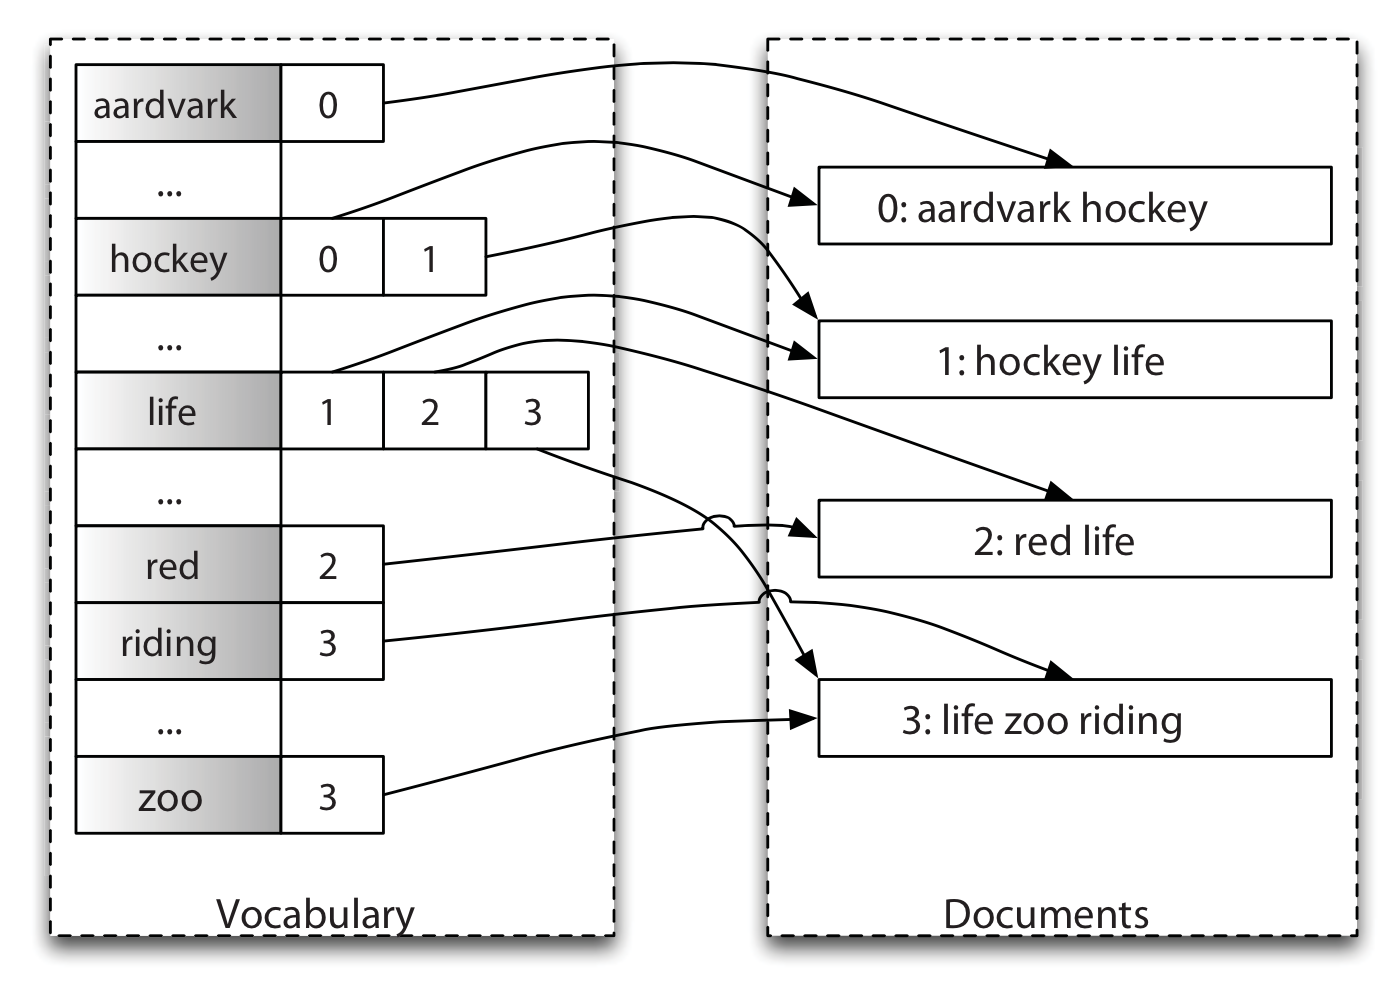
\includegraphics[width=300pt]{inverted_index}
  \caption{Invertirani indeks}
  \label{inverted_index}
\end{figure}

Uz pohranjivanje veza između termova i dokumenata, indeksiranje često uključuje i izračunavanje i spremanje informacija o važnosti termova u odnosu na ostale termove u dokumentu, što je detaljnije objašnjeno u \ref{tfidf}. Ta informacija igra veliku ulogu u omogućavanju tražilici da rangira dokumente po relevantnosti (\cite{taming} str. 42).

\section{Upit}

Nakon indeksiranja tražilica je spremna za upit. Da bi napravio upit, korisnik komunicira kroz neku vrstu korisničkog sučelja, koje prima jedan (``jednostavno pretraživanje'') ili više (``napredno pretraživanje'') upita i vraća odgovarajuću listu dokumenata.

Prije nego tražilica počne pretraživati indeks, sam tekst upita obično prolazi isti postupak obrade kao i dokumenti kada se indeksiraju. Primjerice, ako su tokeni korjenovani u indeksu, onda bi i tokeni iz upita također trebali biti korjenovani. U sljedećim potpoglavljima ćemo navesti dodatne obrade koje tražilica izvršava na samom upitu.

\subsection{Ključne riječi}

Najosnovniji oblik upita je jednostavno nizanje ključnih riječi odvojenih razmakom (slika \ref{keywords}). Tražilice su obično konfigurirane tako da rezultat takvog upita vrati dokumente koji sadržavaju bilo koju ključnu riječ, s time da su dokumenti koji sadrže više ključnih riječi rangirani više. Međutim, ukoliko je potrebna veća preciznost, tražilica može vraćati isključivo dokumente koji sadrže \textit{sve} ključne riječi.

\begin{figure}[H]
  \centering
  
\includegraphics[width=300pt]{keywords}
  \caption{Primjer upisa ključnih riječi}
  \label{keywords}
\end{figure}

\subsubsection{Dodavanje sinonima}

Kada korisnik u polje za pretraživanje upiše ključnu riječ ``pećina'', on bi u rezultatima najčešće htio dobiti i dokumente koji sadrže riječ ``špilja''. Iz tog razloga se često upit proširuje sa sinonimima svake riječi. Na primjer, koristeći booleove operatore, upit ``mračna pećina'' bi se mogao proširiti na ``mračna pećina OR špilja''.

Proširivanje sinonimima se vrši na upitu, a ne na indeksu, jer bi ta količina dodatnih riječi znatno povećala indeks (za \textit{svaku} riječ se dodaju \textit{svi} sinonimi), indeksiranje bi općenito dulje trajalo i indeks bi trebalo obnoviti svaki put kada se lista sinonima ažurira.

\subsubsection{Ispravljanje zatipaka}

Pri unosu upita, često se mogu pojaviti zatipci (tipfeleri); bilo zato što korisnik ne zna kako se neka riječ piše, bilo iz razloga što je korisnik jednostavno pritisnuo krivu tipku na tastaturi i nije to primjetio. Dodatno, zatipci se mogu pojaviti i u tekstu koji se pretražuje.

Kada bi se sve riječi tražile doslovno, upit poput ``New Yrok'' najvjerojatnije ne bi vratio niti jedan rezultat. To nije dobro korisničko iskustvo, tražilica punog teksta bi trebala moći prepoznati ovakve zatipke, i ponuditi korisniku ispravljeni upit (eng. \textit{did you mean}). Isprva se čini da bi bilo najbolje da tražilica automatski pri pretraživanju provjerava za zatipke. Međutim, to u praksi ne bi dobro funkcioniralo, i moglo narušiti kvalitetu vraćenih rezultata. Na primjer, ukoliko je u pretraživanju korišteno korjenovanje, riječ "running" će se korjenovati u "run", te se riječ "runing" u upitu (koja će ostati ista nakon korjenovanja) neće prepoznati kao zatipak, jer je previše različita od riječi "run". Nadalje, ukoliko se u pretraživanju koriste sinonimi, pri upitu će se provjeravati zatipci za svaki od sinonima, te se mogu pronaći tekstovi s riječima koje uopće nisu slične niti jednoj riječi iz originalnog upita (\cite{fuzzy}). Također, ukoliko neki dokument sadržavi zatipak, zbog TF-IDF-a (potpoglavlje \ref{tfidf}) će se taj dokument rangirati više nego onaj bez zatipka, jer je rijeđi. Drugim riječima, kada je u upitu napravljen zatipak, tražilica će u rezultatima favorizirati dokumente koji isto imaju zatipak, što je obrnuto intuiciji jer su dokumenti sa više zatipaka obično manje stručni (\cite{elasticguide} \textit{Scoring Fuzziness}). Zbog toga je bolje za ispravljanje zatipaka napraviti dodatan upit, u kojem su isključene sve ostale značajke (rangiranje, korjenovanje, sinonimi itd.).

Da tražilica može ispraviti zatipke, mora moći prepoznati kada se vjerojatno radi o zatipku, a kada o različitoj riječi. Za to mora znati koliko su neke dvije riječi ``slične''. Postoje tri vrste mjere sličnosti koje su u upotrebi. Prva vrsta je \textit{udaljenost po izmjenama}, od kojih je najpoznatija \textit{Damerau-Levenshteinova udaljenost}. Damerau-Levenshteinova udaljenost mjeri sličnost dviju riječi izračunavanjem minimalnog broja izmjena koje je potrebno napraviti na jednoj riječi da bi se dobila druga. Te izmjene se dijele u 4 vrste: umetanje, brisanje, supstitucija i transpozicija. Umetanje dodaje slovo na bilo koje mjesto unutar riječi, brisanje briše jedno slovo iz riječi, supstitucija zamjenjuje jedno slovo s drugim, a transpozicija zamjenjuje redoslijed dva susjedna slova (\cite{taming} str. 89 i \cite{elasticguide} \textit{Fuzziness}). Što je manji broj takvih izmjena potrebno da bi se jedna riječ transformirala u drugu, to su te dvije riječi sličnije. U praksi se obično ne upotrebljava Damerau-Levenshteinova udaljenost veća od 2. Jedan razlog tome je što bi računanje Damerau-Levenshteinove udaljenosti veće od 2 bilo vremenski preskupo. Drugi razlog je taj što je Damerau uočio da 80\% ljudskih zatipaka imaju Damerau-Levenshteinovu udaljenost 1 (\cite{damerau}), što znači da udaljenost 3 najvjerojatnije više nije rezultat zatipka.

Druga vrsta mjere za sličnost riječi je \textit{n-gram udaljenost}. \textit{n}-gram je bilo koji \textit{n}-člani podniz uzastopnih elemenata nekog niza. \textit{n}-gram udaljenost mjeri sličnost dviju riječi tako da gleda broj njihovih zajedničkih \textit{n}-torki slova (\cite{taming} str. 99). Dvije riječi su sličnije što više zajedničkih \textit{n}-grama imaju. Jedna prednost \textit{n}-gram udaljenosti u odnosu na Damerau-Levenshteinovu jest da \textit{n}-gram udaljenost penalizira greške u prvim slovima više nego u ostalim slovima u riječi (\cite{taming} str. 92). I to je u upravo u skladu sa načinom na koji se zatipci i rade. Naime, autor teksta neće se skoro nikad napraviti zatipak u prvom ili drugom slovu (jer se takva greška lako uoči), već će ga najčešće napraviti u kasnijim slovima. Ako uspoređujemo dvije riječi i postoji razlika u prvom i/ili drugom slovu, tada se najvjerojatnije ne radi o dvije iste riječi od kojih jedna ima zatipak, već o različitim riječima. U praksi se pokazalo da najbolje rezultate daje promatranje zajedničkih \textit{trigrama} (\cite{postgres} \textit{pg\_trgm}).

Osim sličnosti po slovima, postoje i algoritmi za sličnosti među riječima po \textit{zvučnosti}, i to je treća vrsta mjere. Originalni algoritam je \textit{Soundex}, koji funkcionira tako da svakoj riječi pridruži niz znakova, koji označava njenu ``zvučnost'' te se ti znakovi onda mogu uspoređivati. Soundex radi samo za engleski jezik. Soundex je zatim razvijen u \textit{Metaphone}, koji poboljšava algoritam tako da koristi informaciju varijacija i nedosljednosti engleskog jezika da proizvede točniji niz znakova. Sljedeća verzija Metaphonea je nazvana \textit{Double Metaphone}. Glavna stvar koju Double Metaphone dodaje je prva podrška za ne-engleske vrste jezika: slavenski, germanski, keltski, grčki, francuski, talijanski, španjolski i kineski (\cite{metaphone}).

Niti jedna od te tri mjere udaljenosti nije najbolja, te bi svaka tražilica trebala nuditi sve tri mjere, tako da aplikacija može izabrati jednu ili više njih ovisno o načinu na koji žele da se ispravljaju zatipci.

\subsection{Fraze}

Pretpostavimo da radimo aplikaciju koja omogućuje korisnicima da gledaju riječi pjesama. Pretpostavimo sada da korisnik želi iskoristiti tu aplikaciju da pronađe naziv i autora pjesme na temelju fraza koje je zapamtio iz slušanja te pjesme. Ako korisnik upiše te fraze iz pjesme kao običan niz ključnih riječi, postoji vjerojatnost da će rezultati uključivati i druge pjesme koje sadrže te ključne riječi pa možda pjesma koju korisnik traži neće biti na prvom mjestu. S druge strane, kada bi korisnik mogao reći tražilici da se određeni nizovi riječi iz upita nalaze u dokumentima točno tim redoslijedom, broj vraćenih pjesama se može znatno smanjiti (jer je puno manja vjerojatnost da dvije pjesme dijele čitavu frazu) i puno je vjerojatnije da će tražena pjesma biti prvi rezultat.

Niz ključnih riječi može se označiti kao fraza tako da se omeđi dvostrukim navodnicima (slika \ref{phrases}). Tražilica pretražuje dokumente za frazu pomoću \textit{n}-grama. Ranije smo radili s \textit{n}-gramima na razini slova, ali ovdje se \textit{n}-grami koriste na razini riječi. Radi brzine se najprije s manjim \textit{n}-gramima odredi na kojim mjestima je najvjerojatnije da se fraza nalazi te se zatim ispituju zabilježena mjesta (\cite{taming} str. 31).

\begin{figure}[H]
  \centering
  
\includegraphics[width=300pt]{phrases}
  \caption{Primjer upisa fraza}
  \label{phrases}
\end{figure}

\subsection{Booleovi operatori}

Ranije smo spomenuli da za upit ključnim riječima većina tražilica vraća sve dokumente koji sadrže neku od ključnih riječi (s tim da su rangirani više oni koji sadrže više ključnih riječi). Međutim, ako primjerice korisnik želi pronaći sve knjižnice u Zagrebu, htio bi da su rezultati isključivo dokumenti koji sadrže obje riječi ``knjižnica'' i ``zagreb''.

Zato tražilice obično omogućuju da se između ključnih riječi stave tzv. \textit{Booleovi operatori} (slika \ref{boolean}). Operator \textbf{AND} znači da desna i lijeva ključna riječ moraju \textit{obje} biti sadržane u dokumentu, operator \textbf{OR} znači da dokument mora sadržavati \textit{barem jednu} od omeđujućih ključnih riječi, dok operator \textbf{NOT} znači da dokument \textit{ne smije} sadržavati ključnu riječ koja slijedi. Moguće je i korištenje zagrada za gradnju složenijih booleovih izraza.

\begin{figure}[H]
  \centering
  
\includegraphics[width=300pt]{boolean}
  \caption{Primjer booleovih operatora}
  \label{boolean}
\end{figure}

\subsection{Zamjenski znakovi i regularni izrazi}

Naprednijim korisnicima trebalo bi omogućiti maksimalnu preciznost pretraživanja. U tu svrhu može se omogućiti upotreba zamjenskih znakova \textit{?}, koji reprezentira 1 proizvoljan znak, i \textit{*}, koji reprezentira bilo koji broj (uključujući i 0) proizvoljnih znakova (slika \ref{wildcards}). Tako će \textit{bank?} pronaći riječi ``banka'', ``banke'', ``banki'' itd, dok će \textit{bank*} pronaći i riječi kao ``bankama'' i ``bankarstvo''.

\begin{figure}[H]
  \centering
  
\includegraphics[width=300pt]{wildcards}
  \caption{Primjer zamjenskih znakova}
  \label{wildcards}
\end{figure}

Dok ova dva zamjenska znaka daju kontrolu dovoljnu u većini slučajeva, postoje neki (rijetki) slučajevi u kojima je potrebna veća preciznost (npr. pretraživanje programskog kôda). Zato neke tražilice u upitu omogućuju i korištenje regularnih izraza.

\subsection{Specificiranje polja}

Pretpostavimo da korisnik želi kupiti čvrsti disk, ali ne zna točno koji želi. Korisnik otvori \url{www.nabava.net}, i uđe u kategoriju ``Računala > Pohrana podataka > Čvrsti diskovi'' (slika \ref{nabava1}).

\begin{figure}[H]
  \centering
  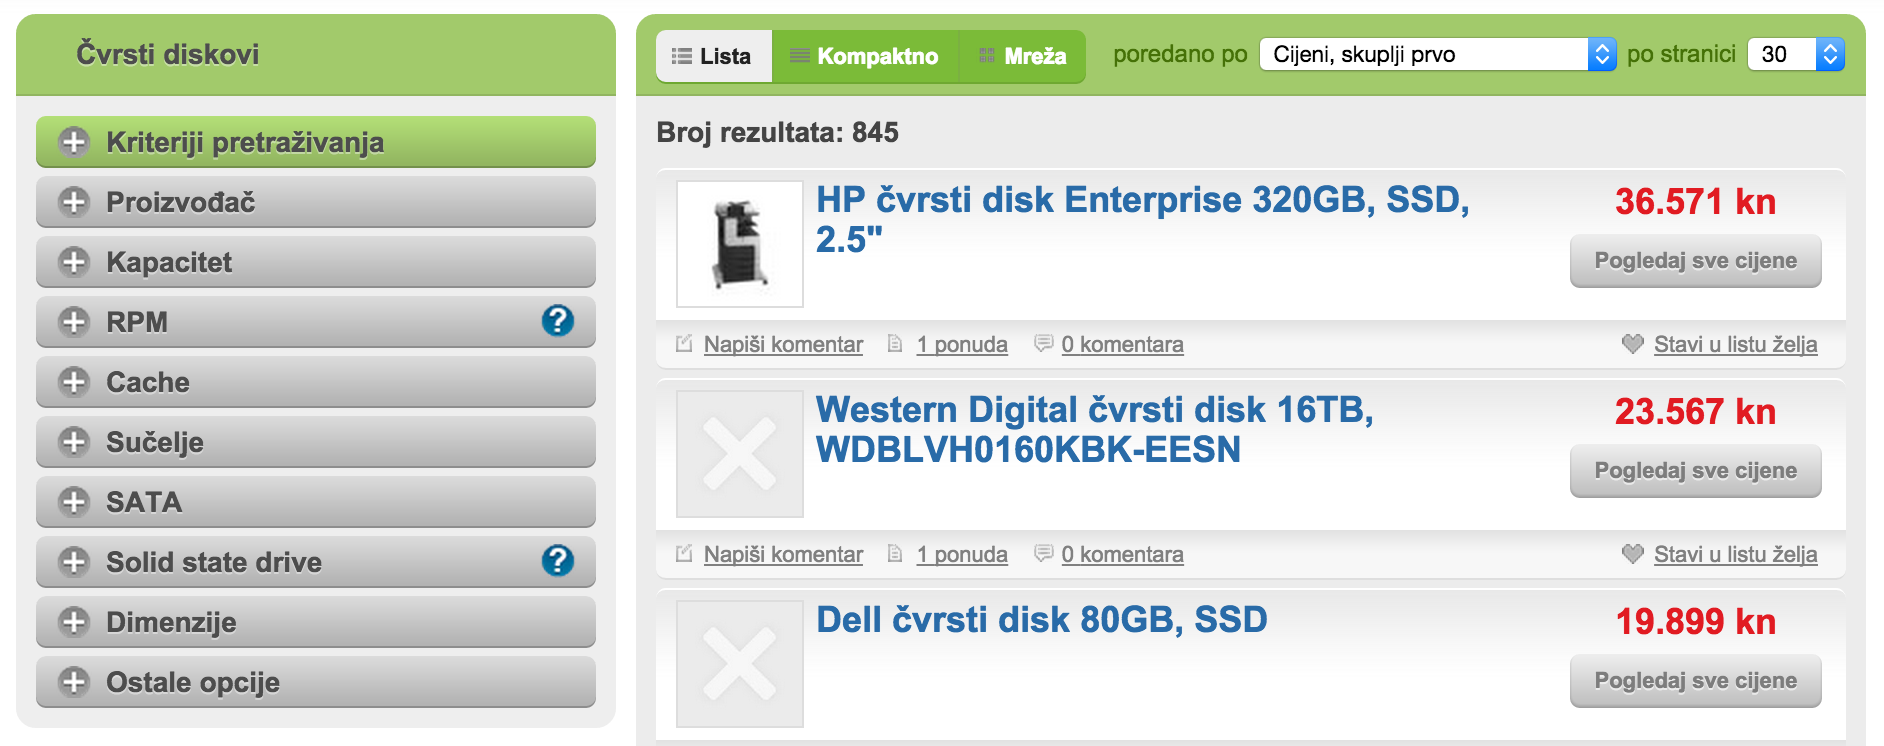
\includegraphics[width=\textwidth]{nabava1}
  \caption{Kategorija ``Čvrsti diskovi'' na \url{www.nabava.net}}
  \label{nabava1}
\end{figure}

Korisnik zatim počne razmišljati koji točno čvrsti disk želi. Prvo, odluči da želi kupiti disk od tvrtke HP i u lijevom izborniku označi da želi da mu se prikažu svi čvrsti diskovi od te kompanije (slika \ref{nabava2}).

\begin{figure}[H]
  \centering
  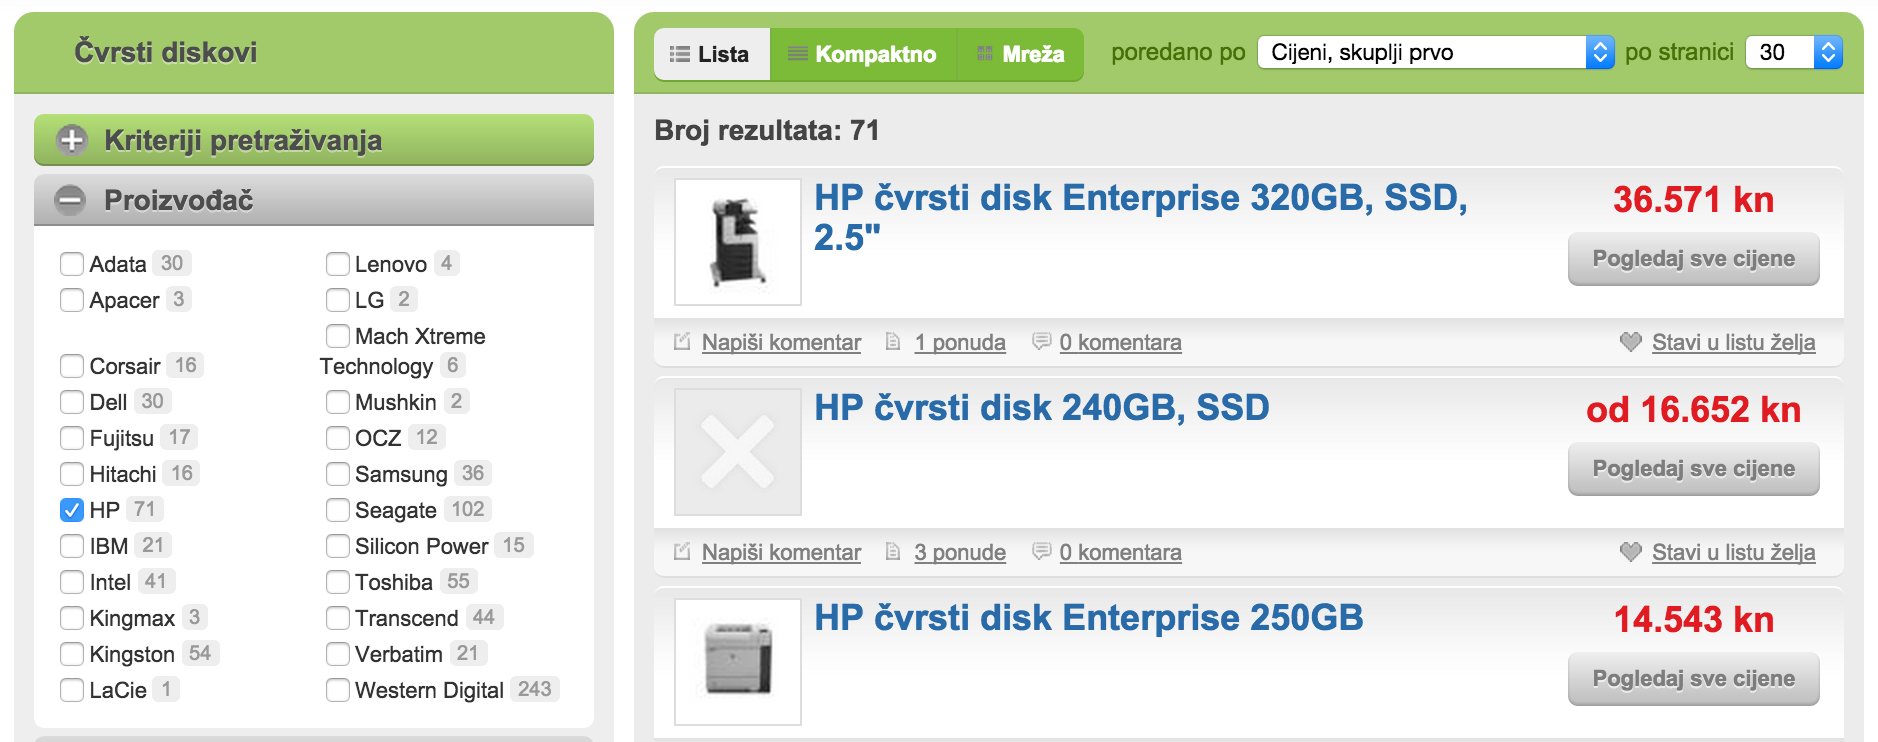
\includegraphics[width=\textwidth]{nabava2}
  \caption{Filtriranje kompanije na \url{www.nabava.net}}
  \label{nabava2}
\end{figure}

Budući da korisnik želi na taj disk uglavnom spremati filmove, odluči da mu treba disk s većim kapacitetom te u lijevom izborniku označi kapacitet ``512GB - 2TB'' (slika \ref{nabava3}).

\begin{figure}[H]
  \centering
  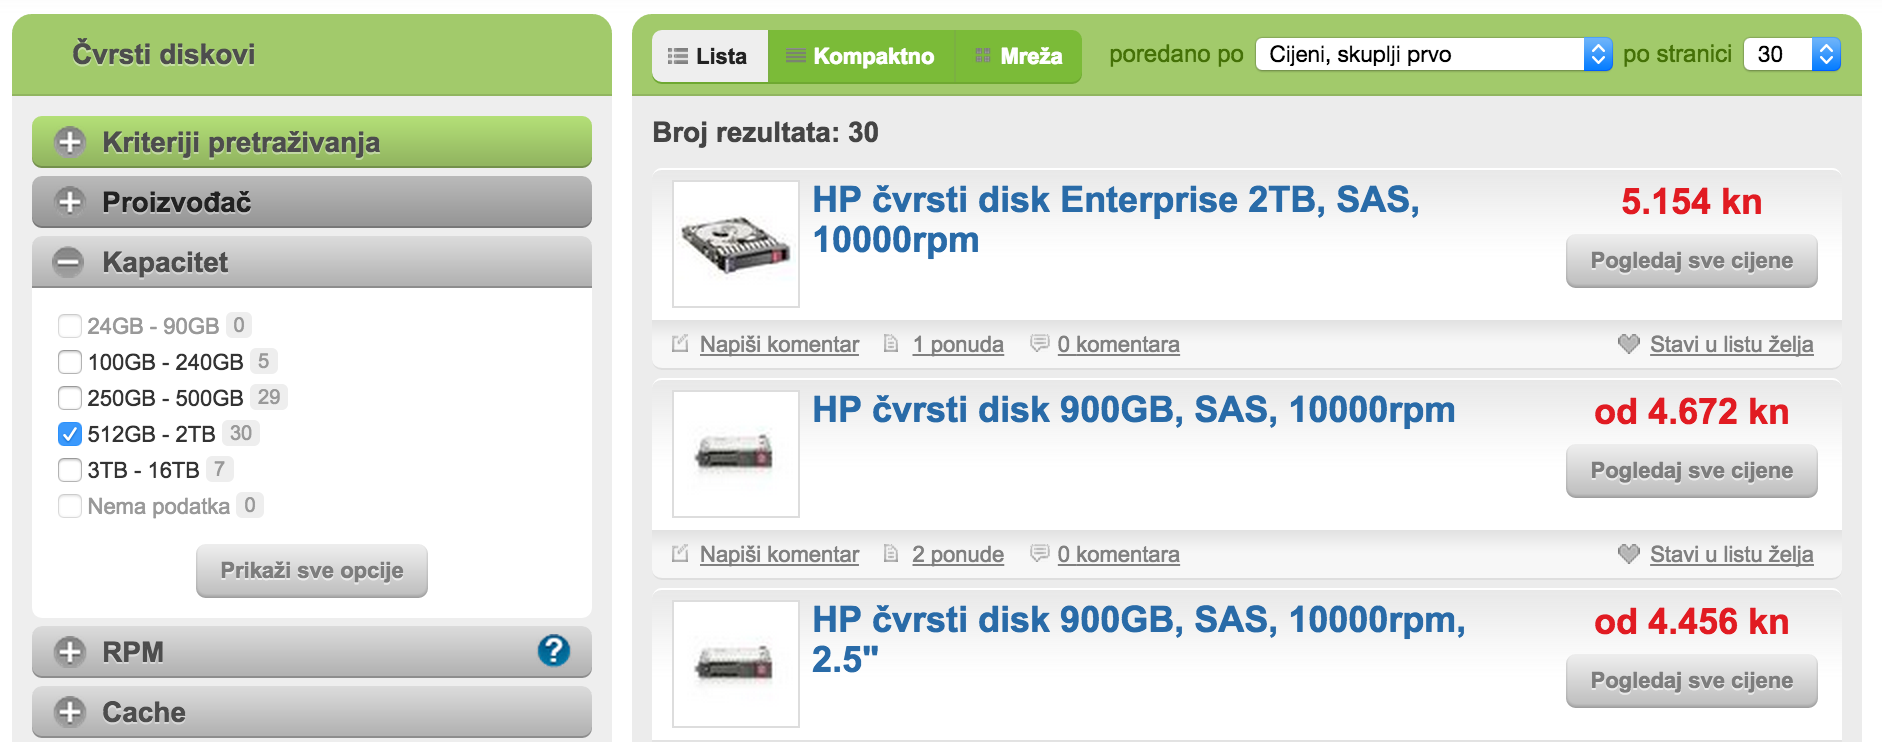
\includegraphics[width=\textwidth]{nabava3}
  \caption{Filtriranje kapaciteta diska na \url{www.nabava.net}}
  \label{nabava3}
\end{figure}

Uz odgovarajuće sortiranje korisnik pronađe željeni disk. Da korisnik nije imao lijevi izbornik koji mu je pomogao filtrirati proizvode po određenim kategorijama, teško bi mogao naći željeni čvrsti disk. U ovom slučaju tekstualno polje ne bi pomoglo, jer korisnik ne zna točno što želi, i ne zna što je dostupno.

Zato tražilice omogućuju i upite koji će pretraživati specifična polja dokumenata. Gornji primjer je slučaj kada su moguće vrijednosti polja već predefinirane korisniku. Generalno, postoje dvije vrste upita po poljima. Jedna vrsta je upisivanje specifične vrijednosti polja, što je pogodno za tekstualna polja kao što su ``autor'' i ``kategorija''. Druga vrsta je specificiranje nekog intervala vrijednosti, što je pogodno za numerička i vremenska polja kao što su ``cijena'' i ``datum rođenja''.

\subsection{Automatsko nadopunjavanje}

Dok korisnik upisuje znakove u polje za upit, aplikacije često otvaraju listu sugestija iz dokumenata koji se nalaze u indeksu, na temelju znakova koje je korisnik trenutno upisao (slika \ref{typeahead}). Najčešće se taj niz znakova uzima kao prefiks. To poboljšava korisničko iskustvo na više načina. Prvo, korisniku to može skratiti količinu tipkanja jer u bilo kojem trenutku može izabrati sugestiju, bez da mora završiti tipkati. Drugo, ako korisnik dobije listu sugestija, onda zna da do sada nije napravio prevelike zatipke. Treće, automatska povratna informacija o korisnikovim upisanim znakovima vodi korisnika da napravi upit koji će sigurno vratiti rezultate.

\begin{figure}[H]
  \centering
  
\includegraphics[width=300pt]{typeahead}
  \caption{Primjer automatskog nadopunjavanja na \url{www.google.com}}
  \label{typeahead}
\end{figure}

Lista sugestija se najčešće dobavlja korištenjem \textit{n}-grama, na sličan način kao kod ispravljanja zatipaka. Najprije se dobavljaju riječi koje sadrže barem jedan zajednički \textit{n}-gram s upitom, a zatim se ta lista rangira po broju zajedničkih \textit{n}-grama (\cite{taming} str. 100).

\section{Rangiranje}

Kada tražilica pretražuje sve dokumente koji ispunjavaju dani upit, potrebno je odrediti koliko je neki dokument ``relevantan'' upitu. Iako je tražilicama obično moguće proslijediti opciju sortiranja rezultata po nekom kriteriju (npr. alfabetski ili po cijeni), odsustvo te opcije podrazumijeva da tražilica vraća rezultate sortirane po ``relevantnosti''.

\subsection{Model vektorskog polja}

Da bismo rangirali dokumente, potrebno je definirati mjeru ``relevantnosti'' upitu. Najprije je potrebno postaviti model u kojem ćemo definirati tu mjeru. Postoji mnogo različitih modela, a mi ćemo promatrati najpopularniji – model vektorskog polja.

Ideja modela vektorskog polja je promatranje dokumenata kao vektore u \textit{n}-dimenzionalnom vektorskom prostoru. Vektorski prostor je definiran tako da svaka dimenzija odgovara jednom tokenu iz skupa svih jedinstvenih tokena iz svih dokumenata. Na primjer, pretpostavimo da imamo kolekciju sljedećih dokumentata:

\begin{compactenum}
  \item ``Ivica Kostelić odnosi pobjedu u skijaškom kupu''
  \item ``Janica Kostelić odnosi pobjedu u svjetskom prvenstvu''
\end{compactenum}

Tada modeliramo ova dva dokumenta kao vektore u $10$-dimenzionalnom vektorskom prostoru (budući da unija tokena iz gornja dva dokumenta čini $10$-člani skup). Budući da su dokumenti zapravo niz tokena, možemo ih promatrati kao vektore u tom vektorskom prostoru kojemu je \textit{k}-ta komponenta jednaka $1$ ako token \textit{k} postoji u dokumentu, ili $0$ ako token ne postoji u dokumentu. Neka numeriramo tokene iz našeg primjera na sljedeći način:

\begin{center}
  \begin{tabular}{@{\enspace}c@{\enspace}c@{\enspace}c@{\enspace}c@{\enspace}c@{\enspace}c@{\enspace}c@{\enspace}c@{\enspace}c@{\enspace}c@{\enspace}}
    1     & 2      & 3        & 4      & 5       & 6 & 7         & 8         & 9    & 10        \\
    ivica & janica & kostelić & odnosi & pobjedu & u & skijaškom & svjetskom & kupu & prvenstvu \\
  \end{tabular}
\end{center}

Tada naša dva dokumenta postaju sljedeći vektori:

\begin{compactenum}
  \item $(1,0,1,1,1,1,1,0,1,0)$
  \item $(0,1,1,1,1,1,0,1,0,1)$
\end{compactenum}

Sada kada smo definirali model vektorskog polja, možemo definirati pojam ``relevantnosti'' dokumenta upitu. Ukoliko gledamo i upit kao vektor u istom vektorskom prostoru, možemo promatrati koliko se upit podudara s dokumentom tako da gledamo kut između ta dva vektora. Ukoliko je kut $0\degree$, znači da imamo potpuno podudaranje. Onda možemo definirati ``relevantnost'' kao kosinus tog kuta, koji će uvijek biti broj između $-1$ i $1$, s time da će biti maksimalan ($1$) upravo kada je kut $0\degree$.

\subsection{Težina riječi}
\label{tfidf}

Da bi se poboljšala kvaliteta tražilice, umjesto samog spremanja $1$ za indikaciju da riječ postoji u dokumentu, tražilice obično spremaju neku vrstu težine koja predstavlja relativnu važnost te riječi u odnosu na ostale riječi.

Najčešći sustav težina koji se koristi je \textit{TF-IDF} (eng. \textit{Term Frequency – Inverse Document Frequency}). Glavna ideja je sljedeća; riječ koja se pojavljuje često u dokumentu je važnija, osim ako se pojavljuje često i u ostalim dokumentima. Drugim riječima, važnost riječi je proprocionalna broju pojavljivanja u dokumentu (TF) i obrnuto proporcionalna općenitom broju pojavljivanja u svim dokumentima (IDF).

U našem primjeru, u prvom dokumentu se riječ ``Ivica'' pojavljuje $1$ put, dok se u drugom dokumentu ne pojavljuje. Dakle njena prosječna frekvencija je $0.5$, iz čega slijedi da je njena težina $TF / IDF = 1 / 0.5 = 2$. S druge strane, riječ ``u'' se u oba dokumenta pojavljuje 1 puta, pa je njena težina $1 / 1 = 1$. Napravimo li to za svaku riječ, prvi dokument postaje

\begin{nscenter}
  \begin{tabular}{c}
    $(1,0,1,1,1,1,1,0,1,0)$ \\
    $\downarrow$            \\
    $(2,0,1,1,1,1,2,0,2,0)$ \\
  \end{tabular}
\end{nscenter}

\subsection{Težina polja}

Pri indeksiranju je moguće nekim poljima dokumenta dati veću težinu. Na primjer, ako se radi o vijestima za novine, naslov članka je najčešće važniji nego tijelo. Tako da, ako dio upita odgovara naslovu, to je puno veći uspjeh nego da odgovara tijelu članka. Stoga davanje određenim poljima veću težinu rezultira boljim rangiranjem.

Osim eksplicitno namještene težine polja, tražilice često automatski daju poljima težinu s obzirom na njihovu duljinu. Naime, ako je neko polje kraće, za njega postoji manja vjerojatnost da ispunjava upit, a i takva polja su najčešće važnija, te im se zato daje veća težina.

\subsection{Blizina riječi}

Kod rangiranja je također korisno promatrati koliko su pronađene ključne riječi međusobno udaljene. Kada su pronađene ključne riječi međusobno bliže, onda je dokument intuitivno relevantniji, stoga tražilice najčešće rangiraju takve dokumente više. Specijalno, ako su pronađene ključne riječi u dokumentu uzastopne, odnosno ako tvore frazu, taj će dokument dobiti veću relevantnost. To znači da, ako je npr. upit jednak naslovu dokumenta, taj dokument će se vrlo vjerojatno rangirati prvi, što odgovara korisnikovim očekivanjima.

\section{Prikaz rezultata}

U ovom potpoglavlju obradit ćemo elemente pretraživanja punog teksta koji su vezani za sami prikaz rezultata.

\subsection{Paginacija}

Ukoliko je broj dokumenata velik, aplikacija najčešće ne želi odmah prikazati sve dokumente jer bi to povećalo vrijeme učitavanja web stranice, a većina rezultata ne bi ni stala na ekran. Iz tog razloga tražilice često uz upit prihvaćaju i opciju (a) koliko dokumenata tražilica treba vratiti (eng. \textit{limit}) i (b) koji prozor rezultata treba vratiti (eng. \textit{offset}). Na taj način aplikacija primjerice može implementirati paginaciju (slika \ref{pagination}).

\begin{figure}[H]
  \centering
  
\includegraphics[width=300pt]{pagination}
  \caption{Paginacija na \url{www.nabava.net}}
  \label{pagination}
\end{figure}

Budući da tražilica najprije mora izračunati relevantnost svih dokumenata, kako bi ih mogla sortirati i vratiti traženi prozor, paginacija najčešće ne ubrzava vrijeme upita direktno. Međutim, ako je ukupni broj dokumenata vrlo velik, paginacijom je moguće znatno smanjiti količinu memorije potrebne za izvršenje upita. Također, ukoliko se upit izvršava preko Interneta, manji broj dokumenata koje tražilica vraća rezultira bržim izvršenjem cijelog HTTP zahtjeva, jer se preko mreže treba prenijeti manja količina podataka.

\subsection{Isticanje}

Mnogo aplikacija, osim vraćenih rezultata, žele prikazati i zašto je pojedini dokument ispunjavao upit. To se postiže isticanjem određenih dijelova dokumenta koji su ispunili upit (slika \ref{highlighting}). Tražilica obično vrati dokumente gdje su dijelovi koji ispunjavaju upit okruženi nekim indikatorom (najčešće je to neki HTML tag, npr. \texttt{<em></em>}), kojeg onda aplikacija prikaže na željen način.

\begin{figure}[H]
  \centering
  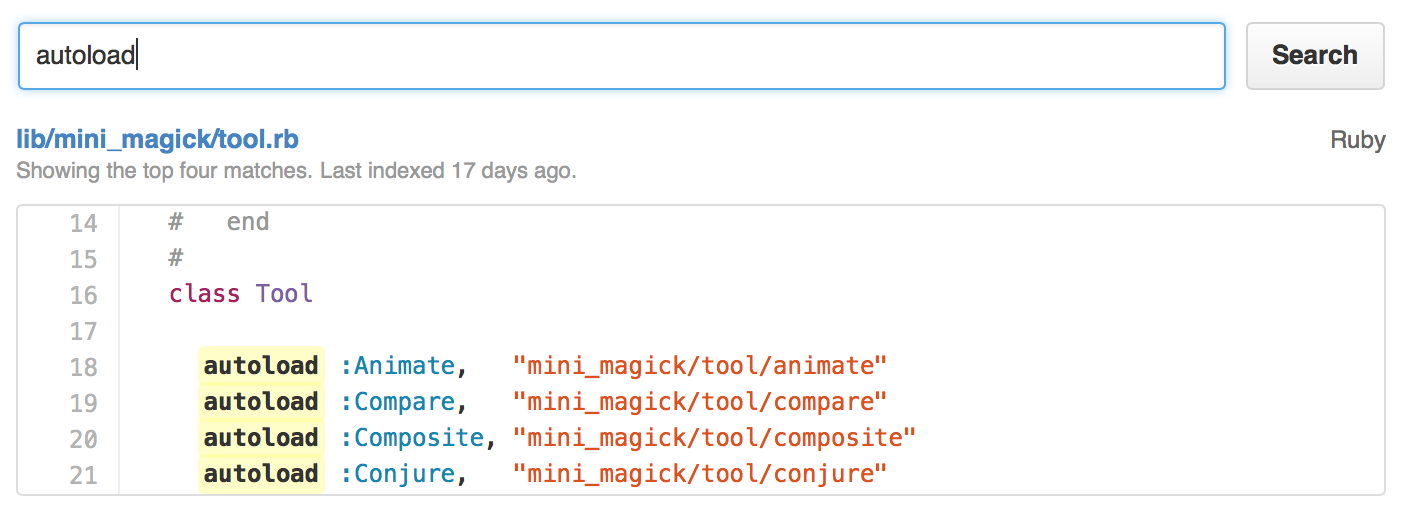
\includegraphics[width=300pt]{highlighting}
  \caption{Isticanje rezultata na \url{http://github.com}}
  \label{highlighting}
\end{figure}

\chapter{Performanse}

Kada gradimo aplikaciju za pretraživanje, s vremenom se broj dokumenata i broj korisnika može znatno povećati. U tom slučaju se performanse pretraživanja mogu znatno smanjiti. Postoje razni aspekti koje možemo mjeriti kako bismo dobili uvid u brzinu pretraživanja:

\begin{compactitem}
  \item \textbf{Propusnost upita} – Broj upita koji sustav može obraditi u nekoj vremenskoj jedinici (npr. broj upita po sekundi).
  \item \textbf{Prosječna brzina upita} – Vrijeme koje prosječnom upitu treba da se obradi.
  \item \textbf{Statistike predmemorije} – Mnogi sistemi spremaju rezultate upita u predmemoriju (eng. \textit{cache}). Korisno je znati koliko je često predmemorija korištena za vrijeme upita, jer ako je rijetko, onda može biti brže isključiti predmemoriju.
  \item \textbf{Veličina indeksa} – Veličina indeksa je obično proporcionalna s vremenom upita.
\end{compactitem}

Prirodan način za ubrzati bilo koji računalni rad je nadogradnja hardvera. To znači da se vrijeme pretraživanja može ubrzati nadogradnjom RAM-a i procesora. Također, upotreba SSD-a (eng. \textit{solid state drive}) može znatno ubrzati vrijeme upita, iako može usporiti ažuriranje dokumenata.

Dok nadogradnja jednog računala može puno pomoći, performanse koje se mogu postići jednim računalom svejedno su ograničene. U jednom trenutku je potrebno distribuirati tražilicu na više računala (\textit{skaliranje}). Tražilice punog teksta podržavaju dvije metode skaliranja:

\begin{compactenum}
  \item \textit{Replikacija} – Jedan indeks koji stane na jedno računalo se može kopirati na više računala. Na taj način se opterećenje može distribuirati po više računala. To je vrlo korisno kada je indeks relativno mali, ali je broj upita vrlo velik.
  \item \textit{Cijepanje} – Jedan indeks se može rascijepati u više dijelova (eng. \textit{shards}) te se svaki dio stavlja na zasebno računalo. Cijepanje indeksa obično interno izvršava tražilica, ali indeks je moguće rascijepati i po logičkom pravilu (npr. po govornom jeziku).
\end{compactenum}

\chapter{Implementacija}

U prethodnim poglavljima obradili smo sve glavne značajke koje bi tražilice punog teksta trebale imati. U ovom poglavlju ćemo napraviti uvod i iznijeti rezultate praktičnog dijela ovog rada.

Praktični dio sastoji se od implementacije obrađenih značajki u svakoj od vodećih tražilica punog teksta, u području softvera otvorenog kôda. Cilj praktičnog dijela je steći znanje o funkcionalnosti svake tražilice kroz direktno iskustvo, te na temelju toga iznijeti prednosti i nedostatke svake tražilice.

Kôd praktičnog dijela napisan je u programskom jeziku Ruby, i nalazi se na \url{https://github.com/janko-m/college-diploma_thesis}. Projekt se sastoji od:

\begin{compactenum}
  \item unificirane implementacije pretraživanja za svaku tražilicu, koja se nalazi u "lib/" direktoriju, i
  \item automatiziranih testova koji za svaku tražilicu testiraju sve značajke iz poglavlja \ref{searching}, a nalaze se u "features/" direktoriju.
\end{compactenum}

\section{Tražilice}

U ovom podpoglavlju navest ću sve tražilice punog teksta koje sam koristio u praktičnom dijelu. Za svaku tražilicu ću najprije dati kratki opis, te ću zatim navesti njihove glavne prednosti i nedostatke.

\subsection{Apache Lucene}

\textit{Apache Lucene} je programska biblioteka sa funkcionalnostima za pretraživanje punog teskta, napisana u Javi i javno distribuirana pod licencom ``Apache License 2.0''. Lucene nije potpuna aplikacija za pretraživanje, već pruža sučelje za to na nižoj razini, kroz Java API (eng. \textit{Application Programming Interface}).

Glavne značajke Apache Lucene uključuju:

\begin{itemize}
  \item mnogo vrsta upita (fraze, zamjenski znakovi, intervali itd.),
  \item pretraživanje po poljima (e.g. naslov, autor itd.),
  \item sortiranje po rangu ili proizvoljnom polju,
  \item pretraživanje po više indeksa s integriranim rezultatima,
  \item paralelno ažuriranje i pretraživanje te
  \item ispravljanje zatipaka.
\end{itemize}

Lucene ugrubo funkcionira na sljedeći način. Prvo se inicijaliziraju dokumenti koji mogu imati jedno ili više polja. Zatim se specificira analizator dokumenata, koji će tokenizirati dokumente po poljima (ne mora se nužno koristiti analizator koji dolazi s Apache Lucene), kodek koji će kodirati i dekodirati iz invertiranog indeksa, i način kako će se indeks spremati (na disku, u memoriji itd.). Nakon toga se može napraviti upit, koji prvo prolazi kroz razne analizatore (fraze, booleovi operatori itd), nakon čega se uspoređuje s indeksom i rezultira pronađenim dokumentima (\cite{lucene} \textit{Introduction to Lucene's APIs}).

Apache Lucene nije bio korišten direktno u praktičnom dijelu (jer on ionako nije namijenjen da se direktno koristi u aplikacijama), ali ga interno koriste Apache Solr i Elasticsearch.

\subsection{Apache Solr}

\textit{Apache Solr} je platforma za pretraživanje punog teksta sagrađena na Apache Lucene, napisana u Javi i javno distribuirana pod licencom ``Apache License 2.0''.

Solr se koristi tako da se pokrene kao web aplikacija te se s njom komunicira preko HTTP protokola (koristeći formate JSON, XML ili CSV). Neki primjeri HTTP zahtjeva na Solr-ovo HTTP API su:

\begin{description}
  \item[\texttt{POST /solr/update}] \hfill \\ Za dodavanje novih, ažuriranje i brisanje postojećih dokumenata iz indeksa.
  \item[\texttt{GET /solr/<collection>/select}] \hfill \\ Za pretraživanje indeksiranih dokumenata
\end{description}

Neke od poznatijih organizacija koje koriste Apache Solr su AT\&T, eBay, Netflix i Disney (uzeto s \url{http://lucene.apache.org/solr/}).

\subsubsection{Prednosti}

Budući da je sagrađen na Apache Lucene, Solr nativno podržava kompleksne upite (booleove operatore, fraze itd.). Također nativno podržava preprocesiranje teskstualnih datoteka, koristeći Apache Tika.

Solr ima nativnu podršku za upravljanje valutama. Na primjer, može odrediti o kojoj se valuti radi iz simbola, i može raditi automatske konverzije (\cite{solr} str. 47).

Automatsko nadopunjavanje je također dobro podržano u Solru. Postoji poseban dio API-a koji je baš namijenjen za tu funkcionalnost (vidi sliku \ref{solr-typeahead}) te je optimiziran za brzinu. Također ima nativnu podršku za ispravljanje zatipaka.

\begin{figure}[H]
  \centering
  \fbox{\texttt{http://localhost:8983/solr/type-ahead?q=appl}}
  \caption{Automatsko nadpounjavanje u Solr-u za početak upita ``appl''}
  \label{solr-typeahead}
\end{figure}

\subsubsection{Nedostaci}

Glavni nedostatak Solra je što ima velik broj modova u kojima se može pokrenuti, te uopće nije jasno koji bi se trebao koristiti. Solr dolazi s primjerima \textit{cloud}, \textit{techproducts}, \textit{dih}, \textit{schemaless}, koji prekonfigurirani s tim različitim modovima (vidi sliku \ref{solr-modes}). U dokumentaciji se potiče pokretanje Solra s tim primjerima, međutim nije jasno zašto su ti oni korisni, jer sadrže puno konfiguracije specifične za te primjere koje korisnik općenito ne želi za svoje dokumente. Ti modovi decentraliziraju Solr i znatno kompliciraju njegovo korištenje, jer se u svakom modu razičite funkcionalnosti implementiraju na različit način (npr. moguće je programatski dodati novi tip dokumenta samo u \textit{SolrCloud} modu).

\begin{figure}[H]
  \centering
  \fbox{\parbox{\textwidth}{\footnotesize\fontfamily{ppl}\selectfont
    \textbf{cloud}: Ovaj primjer pokreće \textit{SolrCloud} klaster od 1-4 čvorova. Pri inicijalizaciji Solr će nam postaviti velik broj pitanja na niskom nivou o tome kakvu želimo internu strukturu Solr-a pokrenuti (eng. \textit{nodes}, \textit{ports}, \textit{shards} itd.).

    \medskip

    \textbf{techproducts}: Ovaj primjer pokreće Solr u \textit{samostalnom} modu, koji ne radi neke specijalne konfiguracije.

    \medskip

    \textbf{dih}: Ovaj primjer pokreće Solr u samostalnom modu sa DataImportHandler-om (DIH) omogućenim, koji može prebaciti podatke iz relacijskih baza u Solr.

    \medskip

    \textbf{schemaless}: Ovaj primjer pokreće Solr u samostalnom modu s vođenom shemom, što dopušta da ažuriramo shemu (npr. polja dokumenata) programatski.
  }}
  \caption{Primjeri s kojima se Solr može pokrenuti (\cite{solr} str. 16)}
  \label{solr-modes}
\end{figure}

Solrov dizajn URL-ova je zastario i nije dosljedan (vidi sliku \ref{solr-urls}), što otežava učenje njegovih funkcionalnosti. To se odražava u njihovom vodiču za početnike, gdje se za indeksiranje dokumenata umjesto običnog alata za rađenje HTTP zahtjeva koristi specijalizirana Java biblioteka koja to ``pojednostavljuje''. Također, Solr ima 2 različite dokumentacije\footnote{\url{https://cwiki.apache.org/confluence/display/solr/Apache+Solr+Reference+Guide} i \url{https://wiki.apache.org/solr/}}, koje opisuju iste komponente, te nije jasno koju bi trebalo čitati.

\begin{figure}[H]
  \centering
  \fbox{\parbox{\textwidth}{
    \texttt{POST /admin/collections?action=CREATE\&name=movies}

    \smallskip

    \texttt{POST /movies/schema}

    \smallskip

    \texttt{GET  /select}
  }}
  \caption{Nedosljednost Solr-ovih URL-ova}
  \label{solr-urls}
\end{figure}

Solr se konfigurira direktnim ažuriranjem konfiguracijskih datoteki koje se nalaze u instalacijskom direktoriju, i nije moguće to raditi preko HTTP API-a. To otežava automatizaciju konfiguracije, jer je teško napisati program koji će ažurirati konfiguraciju. Također, Solr za konfiguraciju koristi zastarjeli format XML (vidi sliku \ref{solr-xml}), koji se teže čita od današnjeg standarda, JSON-a.

\begin{figure}[H]
  \centering
  \begin{lstlisting}[language=XML, frame=single]
<?xml version="1.0" encoding="UTF-8" ?>
<config>
  <luceneMatchVersion>5.0.0</luceneMatchVersion>
  <codecFactory class="solr.SchemaCodecFactory"/>
  <schemaFactory class="ClassicIndexSchemaFactory"/>
  <requestHandler name="/query" class="solr.SearchHandler">
     <lst name="defaults">
       <str name="echoParams">explicit</str>
       <str name="wt">json</str>
       <str name="indent">true</str>
       <str name="df">text</str>
     </lst>
  </requestHandler>
</config>
  \end{lstlisting}
  \caption{Konfiguracija Solra s XML-om}
  \label{solr-xml}
\end{figure}

Solr nema podršku za rangiranje po blizini riječi.

\subsection{Sphinx}

\textit{Sphinx} je platforma za pretraživanje punog teksta, napisana u C++u i javno distribuirana pod licencom ``GNU GPL v2.0''. Sphinx je specijalno dizajniran za dobru integraciju sa SQL bazama podataka i za lako pristupanje skriptnim jezicima.

Aplikacije mogu pristupiti Sphinx-u na tri načina:

\begin{enumerate}[(a)]
  \item preko Sphinx-ove vlastite implementacije MySQL mrežnog protokola, \textit{SphinxQL}-a (ovo je preporučeni način)
  \item preko nativnog API-a za pretraživanje, \textit{SphinxAPI}
  \item kroz MySQL server sa konfiguriranim spremanjem u \textit{SphinxSE}
\end{enumerate}

Neke od poznatijih organizacija koje koriste Sphinx su Tumblr i CouchSurfing (uzeto s \url{http://sphinxsearch.com/info/powered/}).

\subsubsection{Prednosti}

Sphinx ima nativnu integraciju sa svim poznatim SQL bazama (PostgreSQL, MySQL, Microsoft SQL, Oracle itd.), što ga automatski čini iskoristivim za većinu aplikacija. Sve što je potrebno da bi se podaci sinkronizirali je poslati Sphinxu komandu da indeksira (slika \ref{sphinx-indexing}), i on će dograbiti podatke iz SQL baze i staviti u svoj indeks. Sphinx ima više vrsta indeksa, i jedna vrsta je \textit{indeks u realnom vremenu}, koja eliminira potrebu eksplicitnog osvježavanja indeksa jer se oni sami mogu osvježavati (\cite{sphinx} \textit{Real-Time Indices}).

\begin{figure}[H]
  \centering
  \fbox{\texttt{\$ indexer -{}-all -{}-rotate}}
  \caption{Sphinxova komanda u komandnoj liniji za indeksiranje}
  \label{sphinx-indexing}
\end{figure}

Osim standardnih vrsta upita, Sphinx podržava i vrlo napredne vrste. Primjerice, upit ``\textit{pećina SENTENCE medvjed}'' će pronaći sve dokumente u kojima se riječ \textit{pećina} i \textit{medvjed} pojavljuju u istoj rečenici. Slično, upit ``\textit{jabuke PARAGRAPH voćnjak}'' će pronaći sve dokumente u kojima se riječ \textit{jabuka} nalazi u istom paragrafu kao riječ \textit{voćnjak}. Još jedan koristan operator je "MAYBE", koji funckionira kao nekomutativni oblik "OR" operatora; upit ``\textit{jabuka MAYBE kruška}'' neće vratiti dokumente u kojima se pojavljuje riječ \textit{kruška}, a ne pojavljuje se riječ \textit{jabuka}. Zbog Sphinxove napredne sintakse upita potrebno je vrlo malo prevođenja korisničkog upita u domenu Sphinxa (\cite{sphinx} \textit{Extended query syntax}).

Sphinx omogućuje definiranje svojih funkcija rangiranja, koje mogu biti kompozicije postojećih (TF-IDF, blizina riječi itd, vidi sliku \ref{sphinx-ranking}).

\begin{figure}[H]
  \begin{Verbatim}[frame=single]
SELECT * FROM movies WHERE MATCH('future')
OPTION ranker = expr('tf_idf*10 + word_count/2 + user_weight');
  \end{Verbatim}
  \caption{Kombiniranje metoda za rangiranje u Sphinxu}
  \label{sphinx-ranking}
\end{figure}

\subsubsection{Nedostaci}

Sphinx jer potrebno dosta precizno konfigurirati da bi radio dobro (slika \ref{sphinx-configuration}). Na primjer, bez određene inicijalne konfiguracije Sphinx će pri pretraživanju dokumenata učitati cijelu SQL tablicu u memoriju. Doduše, Sphinx ima upute za zaobilaženje tog problema, ali moraju se eksplicitno unijeti u konfiguraciju, što nije prijateljski prema novim korisnicima.

\begin{figure}[H]
  \begin{Verbatim}[frame=single]
searchd {
  listen = 127.0.0.1:9306:mysql41
  log = tmp/searchd.log
  query_log = tmp/searchd.query.log
  pid_file = tmp/sphinx.pid
  workers = threads
}

source movies {
  type = mysql
  sql_host = 127.0.0.1
  sql_user = root
  sql_pass = 
  sql_db = diploma
  sql_port = 3306
  sql_query_range = SELECT MIN(id),MAX(id) FROM documents
  sql_range_step = 1000
  sql_query = SELECT * FROM movies WHERE id>=$start AND id<=$end
  sql_attr_uint = year
}

index movies {
  path = /usr/local/var/data/index
  source = movies
}
  \end{Verbatim}
  \caption{Potrebna konfiguracija Sphinxa}
  \label{sphinx-configuration}
\end{figure}

U Sphinxu ima dva načina indeksiranja, od kojih se svaki konfigurira na drugi način. Prvi način indeksiranja bez konfiguracije zahtijeva da se uvijek iznova indeksiraju svi podaci. To može biti sporo, pa su uvedeni tzv. \textit{delta} indeksi, koji omogućavaju indeksiranje samo dijela dokumenata koji su ažurirani. Međutim, ta postavka se mora konfigurirati na vrlo niskoj razini, a delta indeksi se još moraju ručno spajati s glavnim indeksom, što je sveukupno dosta komplicirano. Zato je Sphinx uveo drugi način indeksiranja, tzv. \textit{indeksi u realnom vremenu}. Međutim, ja nisam uspio postići da rade.

Sphinx nije baš fleksibilan što se tiče podataka koje indeksira. Kada se ažuriraju stupci u nekoj tablici, najčešće je potrebno ažurirati i odgovarajuće deklaracije polja unutar konfiguracije. To komplicira održavanje i često može rezultirati nenadanim greškama.

Sphinx nema podršku za ispravljanje zatipaka i normalizaciju dijakritičkih znakova.

\subsection{PostgreSQL}

PostgreSQL je objektno-relacijska baza podataka, napisana u C-u i javno distribuirana pod licencom ``PostgreSQL License'' (slična BSD i MIT licenci). Iako klasične relacijske baze podataka obično nisu dobre u pretraživanju punog teksta, PostgreSQL se ističe svojim sposobnostima te je validan konkurent.

Neke od poznatijih organizacija koje koriste PostgreSQL su Apple, IMDb, Red Hat i Skype (uzeto s \url{http://www.postgresql.org/about/users/}).

\subsubsection{Prednosti}

Najčešća arhitektura aplikacija se sastoji od glavne, relacijske baze, te se za pretraživanje punog teksta koristi zaseban softver. Ako je ta glavna baza PostgreSQL, moguće je njega koristiti za pretraživanje punog teksta umjesto zasebnog softvera. To znači da nije potrebno konstantno sinkronizirati dokumente između dva softvera, te će indeks uvijek biti najažurniji. Također, pretraživanje punog teksta se u tom slučaju lakše integrira u aplikaciju, i programerski tim koji razvija aplikaciju ima jedan softver manje za održavati.

Postgres se odlikuje po naprednoj tokenizaciji. Osim standardnih vrsta tokena (riječi i brojevi), Postgres sprema u zasebne tokene i emailove, linkove i još mnogo drugih tipova objekata.

\subsubsection{Nedostaci}

Glavni nedostatak Postgresa je što, u usporedbi s ostalim tražilicama punog teksta, daje funkcionalnost na puno nižoj razini. Velik broj osnovnih tipova upita i funkcionalnosti je teško prevesti u domenu Postgresa.

Primerice, Postgres ne prepoznaje booleove upite kakve bi ih korisnik napisao; on zahtijeva da između svake riječi postoji operator. Nema ni direktnu podršku za fraze, nego fraze treba ekstrahirati iz upita i staviti u dodatan SQL upit (slika \ref{postgres-phrases}). Nadalje, Postgres ima funkciju za sličnost dviju riječi, ali ju je nemoguće iskoristiti za ispravljanje zatipaka, osim kada je upit jedna riječ (\cite{goodenough}). Također, Postgres nema podršku za TF-IDF metodu rangiranja.

\begin{figure}[H]
  \begin{Verbatim}[frame=single]
SELECT * FROM movies WHERE content @@ 'future'
AND plot ILIKE '%time travel%';
  \end{Verbatim}
  \caption{Imitiranje fraznog pretraživanja u Postgresu}
  \label{postgres-phrases}
\end{figure}

Pretraživanje kroz više tablica (preko stranih ključeva) se u Postgresu ne može indeksirati. Jedan način kako se to može zaobići je indeksiranjem i pretraživanjem svake tablice posebno, te spajanjem rezultata pomoću stranih ključeva. Međutim, tada je vrlo teško izračunati sveukupnu relevantnost glavnog dokumenta. Drugi način kako se to može zaobići jest denormalizacijom baze. Međutim, to narušava dizajn baze podataka i otežava čuvanje integriteta i generalno održavanje.

Postgres ne podržava normalizaciju dijakritičkih znakova u kombinaciji s korjenovanjem, kada se koristi jezik kojemu su dijakritički znakovi dio gramatike (npr. hrvatski). To je zato što se zbog tehničkih nedostataka normalizacija dijakritičkih znakova može izvršiti jedino prije korjenovanja. I tada bi sve riječi u trenutku korjenovanja bile bez dijakritičkih znakova, pa rječnik korišten za korjenovanje ne bi velik broj riječi uopće mogao prepoznati kao hrvatske te ih ne bi korjenovao. Čak i da nema ovog nedostatka, normalizacija dijakritičkih znakova se nativno ne može indeksirati, jer ju Postgres nije odgovarajuću funkciju \texttt{unaccent()} označio kao IMMUTABLE, što tu značajku čini neupotrebljivom (slika \ref{postgres-unaccent}).

\begin{figure}[H]
  \begin{Verbatim}[frame=single]
CREATE INDEX movies_index ON movies USING gin(unaccent(title));
# ERROR: functions in index expression must be marked IMMUTABLE
  \end{Verbatim}
  \caption{Nemogućnost indeksiranja normalizacije dijakritika u Postgresu}
  \label{postgres-unaccent}
\end{figure}

Općenito je u Postgresu vrlo teško pravilno indeksirati podatke za pretraživanje punog teksta. Potrebno je raditi funkcije u PL/pgSQL-u (posebni programski jezik za Postgres) da se spremi obrađeni tekst u posebni stupac, kojih treba biti više ako će biti više načina pretraživanja, i ti stupci se onda trebaju ažurirati kada se podaci promijene pomoću okidača (slika \ref{postgres-indexing}).

\begin{figure}[H]
  \begin{Verbatim}[frame=single]
CREATE FUNCTION movies_trigger() RETURNS trigger AS $$
begin
  new.content :=
     setweight(to_tsvector(coalesce(new.title,'')),      'A') ||
     setweight(to_tsvector(coalesce(new.year::text,'')), 'A') ||
     setweight(to_tsvector(coalesce(new.plot,'')),       'C') ||
     setweight(to_tsvector(coalesce(new.episode,'')),    'C');
  return new;
end
$$ LANGUAGE plpgsql;

CREATE TRIGGER movies_tsv BEFORE INSERT OR UPDATE
ON movies FOR EACH ROW EXECUTE PROCEDURE movies_trigger();
  \end{Verbatim}
  \caption{Pravilno automatsko indeksiranje punog teksta u Postgresu}
  \label{postgres-indexing}
\end{figure}

\subsection{Elasticsearch}

Elasticsearch je distribuirana platforma za pretraživanje punog teksta i analitiku u realnom vremenu, sagrađena na Apache Lucene. Napisana je u Javi i javno distribuirana pod licencom "Apache License 2.0". Elasticsearch je \textit{dokumentno-orijentirana} baza podataka, što spada u tzv. \textit{NoSQL} tipove baza (naziv dolazi iz činjenice da se s takvim bazama ne komunicira SQL jezikom). Slika \ref{elasticsearch} ilustrira analogiju između elemenata Elasticsearch-a i relacijskih baza.

\begin{figure}[H]
  \centering
  \begin{tabular}{lllllllll}
    RDBMS         & $\Rightarrow$ & Baze    & $\Rightarrow$ & Tablice & $\Rightarrow$ & Redovi    & $\Rightarrow$ & Stupci \\
    Elasticsearch & $\Rightarrow$ & Indeksi & $\Rightarrow$ & Tipovi  & $\Rightarrow$ & Dokumenti & $\Rightarrow$ & Polja  \\
  \end{tabular}
  \caption{Analogija između dokumentno-orijentiranih i relacijskih baza}
  \label{elasticsearch}
\end{figure}

Kao i Apache Solr, Elasticsearch se također sastoji od web aplikacije s kojom se komunicira preko HTTP protokola, preko JSON formata.

\begin{description}
  \item[\texttt{PUT /<namespace>/<type>/<id>}] \hfill \\ Za dodavanje novih, ažuriranje postojećih dokumenata u indeksu
  \item[\texttt{GET /<namespace>/<type>/<id>}] \hfill \\ Za dobivanje indeksiranih dokumenata
  \item[\texttt{GET /<namespace>/<type>/\_search}] \hfill \\ Za pretraživanje indeksiranih dokumenata
  \item[\texttt{DELETE /<namespace>/<type>/<id>}] \hfill \\ Za brisanje indeksiranog dokumenta
\end{description}

Neke od poznatijih organizacija koje koriste Elasticsearch su Wikipedia, The Guardian, Stack Overflow i GitHub (\cite{elasticguide} \textit{Getting Started}).

\subsubsection{Prednosti}

HTTP API Elasticsearcha je vrlo napredan i opsežan. Primjerice, cijelo administriranje je moguće provoditi isključivo preko HTTP API-a. Također, arhitektura i dizajn URL-ova su moderni i slijede najbolje prakse – \textit{REST}\footnote{\url{https://www.ics.uci.edu/~fielding/pubs/dissertation/rest_arch_style.htm}}. Međutim, HTTP API je samo jedan način komuniciranja s Elasticsearchom. Ukoliko je aplikacija koja koristi Elasticsearch napisana u Javi ili jeziku koji može komunicirati sa Javom, umjesto HTTP API-a moguće je koristiti Java API direktno (što je brže).

Za razliku od većine tražilica punog teskta, Elasticsearch sam upravlja replikacijama i cijepanju u skladu s količinom i frekvencijom zahtjeva. To je velika prednost, jer smanjuje količinu potrebnog administriranja, i čini skaliranje na više računala jednostavnijim.

Elasticsearch također ima ugrađenu podršku za kontrolu paralelnih zahtjeva. Općenito, kada dva korisnika žele ažurirati isti dokument u isto vrijeme, može se dogoditi da promjene jednog korisnika prebrišu promjene drugog. Elasticsearch to rješava tzv. optimističnim zaključavanjem, koje se sastoji od toga da svaki dokument ima svoju verziju (koja se inkrementira pri svakom ažuriranju). Tada aplikacija može spriječiti korisnika da ažurira jednu verziju dokumenta ako se u međuvremenu dokument ažuririrao i dobio drugu verziju (\cite{elasticguide} \textit{Data In, Data Out}).

Elasticsearch ima dio API-a koji pruža veliku razinu introspekcije u sveukupno funkcioniranje sustava. Instalacija Elasticsearcha također dolazi i sa web aplikacijom koja vizualno prikazuje to stanje s grafovima, i koja koristi taj API (slika \ref{elastic-monitoring}).

\begin{figure}[H]
  \centering
  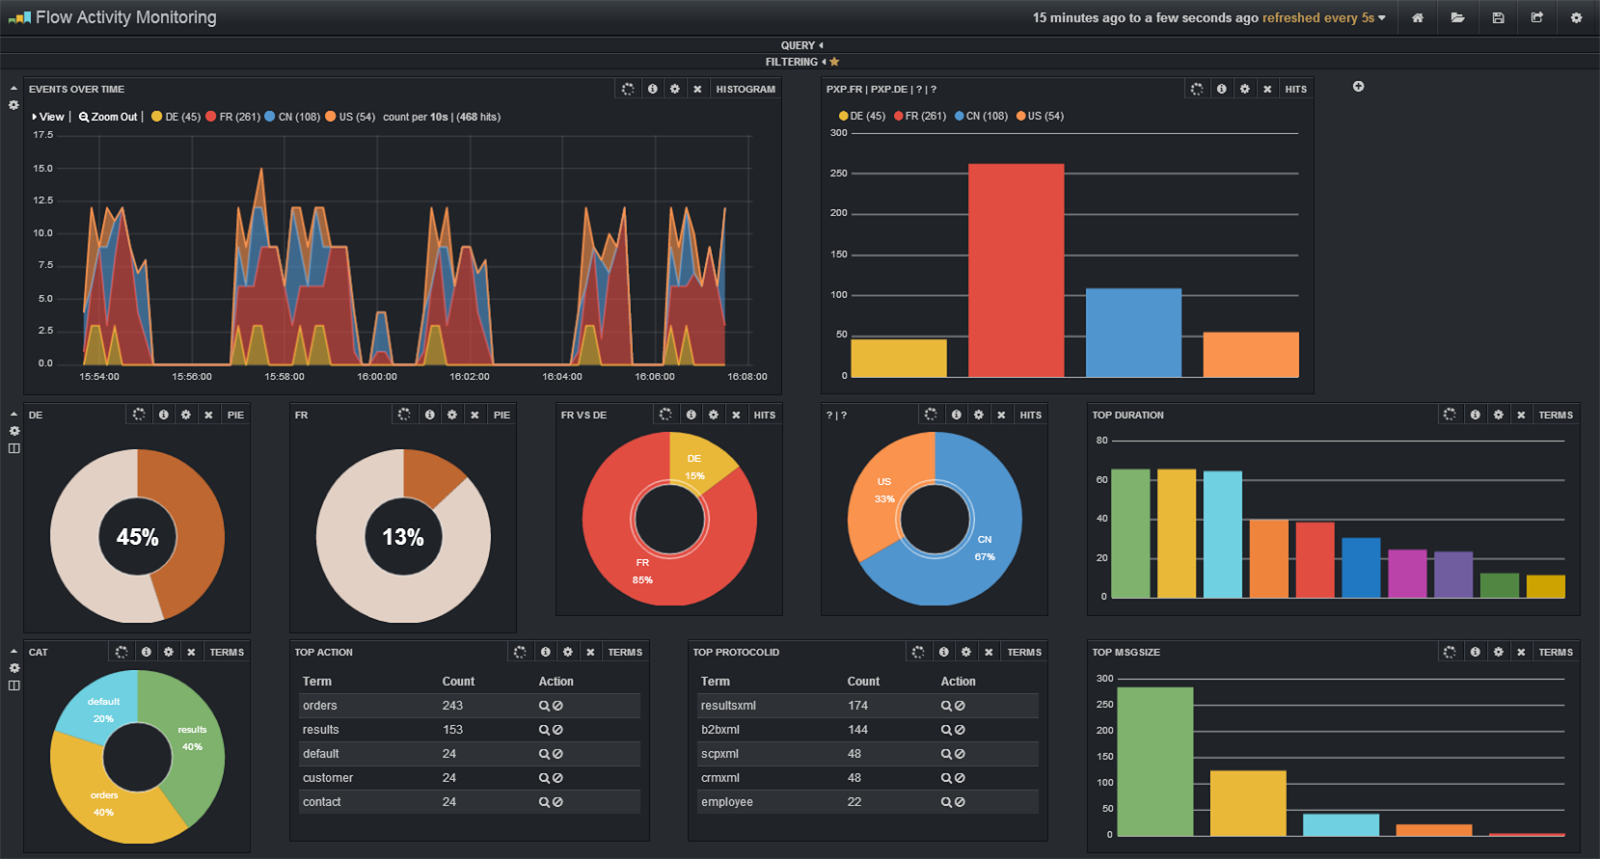
\includegraphics[width=\textwidth]{elastic-monitoring}
  \caption{Aplikacija za nadgledanje Elasticsearcha}
  \label{elastic-monitoring}
\end{figure}

Elasticsearch nativno podržava složene upite (booleovi operatori, fraze, specificiranje polja itd.), te nije potrebno posebno prevoditi dolazeće upite. Osim složenih upita, Elasticsearch podržava i jednostavne upite koji se mogu međusobno kombinirati (slika \ref{elastic-query}). Tako je, na primjer, moguće izvršiti neku vrstu upita te mu dodati upit koji nalazi slične dokumente. Tada će rezultati biti kombinacija ta dva upita, danim redoslijedom (\cite{elasticref} \textit{Search APIs}). Elasticsearch također nativno podržava preprocesiranje tekstualnih datoteki, koristeći Apache Tika.

\begin{figure}[H]
  \centering
  \begin{Verbatim}[frame=single]
"query": {
  "query_string": {
    "query": "back to the future",
    "default_operator": "AND"
  },
  "boosting": {
    "positive": {
      "term": {"_all": "time travel"}
    }
  }
}
  \end{Verbatim}
  \caption{Kombiniranje vrsta upita u Elasticsearchu}
  \label{elastic-query}
\end{figure}

Elasticsearch ima nativno podržanu funkcionalnost automatskog nadopunjavanja, koje je vrlo konfigurabilno i brzo. Također ima i mogućnost ispravljanja zatipaka, na puno različitih načina. Moguće je uz normalan upit automatski napraviti i \textit{fuzzy} upit, a može se i ponuditi ispravljeni upit koji pruža \textit{did you mean} iskustvo.

\subsubsection{Nedostaci}

Elasticsearch nema nativnu podršku za rangiranje rezultata s obzirom na blizinu pronađenih riječi iz upita, što može smanjiti relevantnost rezultata. Međutim, postoji način da se ta funkcionalnost djelomično postigne. Nakon originalnog upita, moguće je ``popraviti'' relevantnost vraćenih dokumenata ponovnim izvršavanjem istog upita, ali ovaj puta ga tretirajući kao frazni upit s olabavljenim zahtjevom razmaka između riječi (u bilo kojem smjeru, tako da se riječi iz upita ne moraju u dokumentu pojaviti danim redoslijedom) (\cite{elasticguide} \textit{Proximity Matching}). Tako se npr. može popraviti relevantnost svih dokumenata u kojima se riječi iz upita pojavljuju u međusobnoj udaljenosti od unutar 100 riječi. Ta metoda će funkcionirati za jednostavne upite, ali neće za složene (jer se u ovoj metodi cijeli upit tretira kao fraza, pa će se npr. booleovi operatori shvaćati doslovno kao riječi).

\chapter{Komercijalne tražilice}

Do sada smo pričali o tražilicama punog teksta koje se mogu koristiti za vlastite web aplikacije, ali samo o onima otvorenog kôda. Međutim, moguće je koristiti i postojeće komercijalne tražilice (Google, Bing itd.) unutar vlastite web aplikacije. Iako smo u uvodu spomenuli da komercijalne tražilice više najčešće nisu potrebne, one još uvijek imaju neke prednosti nad besplatnima. Za usporedbu ćemo uzeti Google tražilicu, budući da je ona daleko najpopularnija od svih komercijalnih (slika \ref{google}).

\begin{figure}[H]
  \centering
  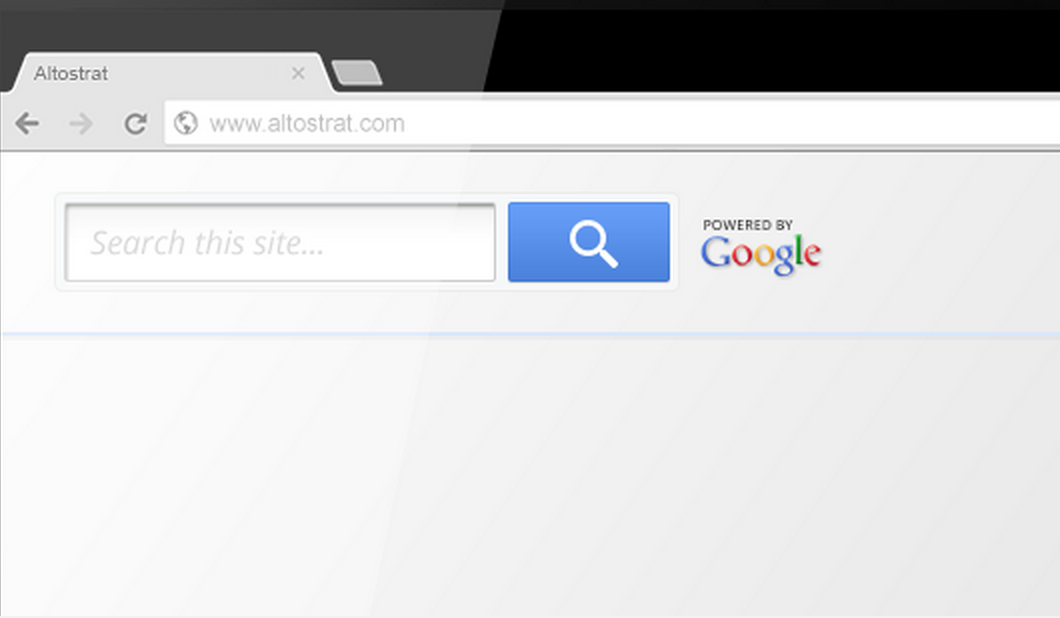
\includegraphics[width=300pt]{google}
  \caption{Google tražilica integrirana u neku web aplikaciju}
  \label{google}
\end{figure}

Glavne značajke integrirane Google tražilice su:

\begin{compactitem}
  \item mogućnost oblikovanja dizajna rezultata i polja za pretraživanje, uključujući i dodavanje vlastitih slika,
  \item pretraživanje kroz različite jezike (moguće je pronaći tekst na jednom jeziku s upitom napisanim na drugom jeziku),
  \item rangiranje dokumenata po datumu zadnjeg ažuriranja,
  \item XML API za maksimalnu fleksibilnost prikaza rezultata,
  \item kategoriziranje dokumenata te omogućavanje korisnicima da filtriraju po tim kategorijama,
  \item mogućnost pretraživanja slika,
  \item rezultati bez reklama,
  \item indeksiranje na zahtjev, npr. kada se neki URL promjeni,
  \item podrška za sinonime i akronime te
  \item mogućnost promoviranja sadržaja kod automatskog nadopunjavanja (\cite{google}).
\end{compactitem}

Glavna prednost integrirane Google tražilice je da Google ima naprednu, poznatu i intuitivnu sintaksu za upite već gotovu. Stoga s Google tražilicom korisnici mogu pisati sve one tipove upita na kakve su već navikli. Također, podrška za korjenovanje, sinonime, akronime i normalizaciju dijakritičkih znakova iz svih jezika je već ugrađena u tražilicu, pa nije potrebno ništa podešavati.

Glavni nedostatak Google tražilice je da ne omogućava potpunu fleksibilnost vraćanja i prikaza rezultata. Google je vrlo dobar u analiziranju HTML stranice i izdvajanju bitnih dijelova teksta. Što web stranica ima bolje strukturiran HTML, to će Google bolje napraviti svoju analizu. Međutim, on nikad neće znati od kojih se točno polja sastoje dokumenti na stranici (i kojih sve tipova dokumenata ima). To znači da u rezultatima vraćenim XML API-om nećemo moći dobiti dobro strukturirane podatke, što ograničava fleksibilnost prikaza rezultata.

\chapter{Zaključak}

Apache Solr nastoji biti gotova platforma za pretraživanje punog teksta, te ima puno ugrađenih naprednih funckonalnosti. Međutim, za vrijeme razvijanja počeo se granati u previše različitih smjerova, od kojih niti jedan nije postao onaj pravi, i nije imao prioritet ostati moderan. To otežava učenje i korištenje Solra, i ne vjerujem da će se još dugo koristiti.

Sphinx se htio usko vezati za postojeće relacijske baze, s ciljem da što više pojednostavni indeksiranje. Međutim, Sphinx se nije orijentirao na lako korištenje, već će on raditi jako dobro tek kada se pažljivo i detaljno konfigurira. Vjerujem da će tvrtke koje su do sada uložile vremena u Sphinx ostati pri njemu, ali mislim da će Sphinx teže zainteresirati nove korisnike.

PostgreSQL je, uz već postojeću odličnu funkcionalnost najnaprednije relacijske baze podataka otvorenog kôda, odlučio pružiti korisnicima i mogućnosti pretraživanja punog teksta. Dok je vrlo pogodno imati tu funkcionalnost direktno u glavnoj bazi podataka, razina na kojoj se s tim alatima mora raditi je preniska za naprednije pretraživanje punog teksta. PostgreSQL će se još dugo nastaviti razvijati kao relacijska baza podataka, ali mislim da se podrška za pretraživanje punog teksta više neće puno mijenjati.

Elasticsearch kao dokumentno-orijentirane baza podataka sadrži vrlo napredne vrste upita i indeksiranja koji se mogu kombinirati, a istovremeno ostaje vrlo lak za korištenje i skaliranje, favorizirajući konvenciju preko konfiguracije. Zbog izvrsne dokumentacije i držanja svog kôda na GitHub-u (web aplikaciji koja omogućava svakome da prati i sudjeluje u razvijanju softvera), vjerujem da će Elasticsearch među softverima otvorenog kôda nastaviti biti najbolja platforma za pretraživanje punog teksta.

\begin{thebibliography}{99}
  \bibitem{taming} G. S. Ingersoll, T. S. Morton, A. L. Farris, \textit{Taming Text: How to Find, Organize, and Manipulate It}, Manning Publications Co, New York, 2013.
  \bibitem{lucene} \textit{Apache Lucene™ 5.0.0 Documentation}, \url{http://lucene.apache.org/core/5_0_0/index.html} (travanj, 2015)
  \bibitem{solr} \textit{Apache Solr Reference Guide}, \url{http://ftp.carnet.hr/misc/apache/lucene/solr/ref-guide/apache-solr-ref-guide-5.0.pdf} (travanj, 2015)
  \bibitem{sphinx} \textit{Sphinx 2.2.6-release reference manual}, \url{http://sphinxsearch.com/docs/archives/2.2.6/} (travanj, 2015)
  \bibitem{postgres} \textit{PostgreSQL 9.4.1 Documentation}, \url{http://www.postgresql.org/docs/9.4/static/index.html} (travanj, 2015)
  \bibitem{elasticguide} C. Gormley, Z. Tong, \textit{Elasticsearch - The Definitive Guide}, \url{http://www.elastic.co/guide/en/elasticsearch/guide/current/index.html} (travanj, 2015)
  \bibitem{elasticref} C. Gormley, Z. Tong, \textit{Elasticsearch reference – 1.5}, \url{http://www.elastic.co/guide/en/elasticsearch/reference/1.5/index.html} (travanj, 2015)
  \bibitem{metaphone} \textit{Metaphone}, \url{http://en.wikipedia.org/wiki/Metaphone} (travanj, 2015)
  \bibitem{fuzzy} A. Cholakian, \textit{How to Use Fuzzy Searches in Elasticsearch}, \url{https://www.found.no/foundation/fuzzy-search/} (travanj, 2015)
  \bibitem{damerau} \textit{Damerau–Levenshtein distance}, \url{http://en.wikipedia.org/wiki/Damerau-Levenshtein_distance} (travanj, 2015)
  \bibitem{goodenough} R. Belaid, \textit{Postgres full-text search is Good Enough!}, \url{http://blog.lostpropertyhq.com/postgres-full-text-search-is-good-enough/} (travanj, 2015)
  \bibitem{google} \textit{Google Site Search}, \url{https://www.google.com/work/search/products/gss.html} (travanj, 2015)
\end{thebibliography}

\pagestyle{empty}

\begin{sazetak}
  Zbog sve većeg rasta digitalnih informacija, potrebne su napredne metode pretraživanja velikih količina teksta. Tradicionalno su relacijske baze podataka obavljale posao pretraživanja informacija, ali one su dobre samo za strukturirano i diskretno pretraživanje. Pretraživanje punog teksta zahtijeva napredne tehnike obrade teksta, kako bi se mogao dati odgovor na pitanje \textit{koliko} dani upit odgovara nekom dokumentu.

  Pretraživanje punog teksta zahtijeva da se tekst informacija unaprijed obradi, kako bi se moglo omogućiti što brže izvršavanje upita. Tako se tekst najprije rastavlja na rečenice, a rečenice na tokene, što svodi pretraživanje teksta na pretraživanje liste tokena. Zatim se tim tokenima sva slova pretvore u mala i normaliziraju se dijakritički znakovi, što pojednostavljuje potrebne znakove za upit. Nakon toga se eliminiraju sve stop-riječi (riječi koje ne donose semantičko značenje) te se sve riječi korjeniziraju, što omogućava da riječ iz upita pronađe sve dokumente koji sadrže bilo koju varijaciju te riječi (npr. po brojnosti i padežu). Zatim se ta obrađena lista tokena sprema u strukturu koja se zove \textit{indeks}, i koja se koristi pri pretraživanju.

  Nakon indeksiranja moguće je raditi upite na stvoreni indeks. Sam tekst upita najprije prolazi kroz istu transformaciju kao i indeks, s time da se još svaka riječ proširuje njenim sinonimima, da bi se pronašao što veći broj relevantnih dokumenata. Zatim se tekst upita analizira za potencijalne fraze (niz riječi unutar dvostrukih navodnika), booleove operatore, zamjenske znakove i regularne izraze. U upit je moguće uključiti i strukturirano pretraživanje specificiranjem polja. Za vrijeme upisivanja upita, korisno je korisniku ponuditi prozor koji automatski predviđa više nastavaka njegovog upita. Za vrijeme izršavanja upita je dobro i tolerirati neke eventualne zatipke.

  Konačno, budući da kod ovakvih pretraživanja često velik broj dokumenata odgovara upitu, potrebno je rangirati dokumente po relevantnosti, na koju se može utjecati na mnogo načina. Osim automatske relevantnosti temeljene na broju pojavljivanja ključnih riječi u dokumentu, moguće je odrediti da su neka polja dokumenta važnija od drugih (npr. naslov), pa rangirati upit koji je pronađen u naslovu više. Također je dobro rangirati i dokumente po redoslijedu i međusobnoj blizini riječi iz upita.

  Dugo vremena su se za pretraživanje unutar web stranica koristile komercijalne tražilice poput Googlea. Međutim, kroz zadnjih 5 godina razvio se velik broj tražilica punog teksta otvorenog kôda. Najpoznatije su Apache Solr, Sphinx, PostgreSQL (koji je dobio podršku za pretraživanje punog teksta) i Elasticsearch. Kroz testiranje i analizu značajki pokazalo se da je među njima prevladao Elasticsearch.

  Velik broj ljudi svakidašnje koristi kvalitetne tražilice kao što je Googleova, i postaje zadatak ostalih web stranica da kvalitetu svojeg pretraživanja pokušaju što više približiti tom standardu.
\end{sazetak}

\begin{summary}
  Because of increasing growth of digital information, advanced methods of searching large amounts of text are required. Traditionally relational databases were doing the job of searching information, but they are good only for structured and discrete searching. Full-text search requires advanced methods of text processing, so that the question \textit{how much} the given query matches a document can be answered.

  Full-text search requires that the text is processed upfront, so that maximum query execution speed can be achieved. The text is first split into sentences, then each sentence is tokenized, which enables searching text to become searching a list of tokens. Afterwards all tokens are downcased and have their diacritics normalized, which simplifies the character set needed for queries. Then stopwords (words that don't bring additional meaning) are removed from the token list and stemming is applied for each token, which enables a keyword in the query to find all documents with any variation of that keyword (e.g. plural or singular). Finally the processed list of tokens are saved in a structure called \textit{the index}, which is then used for searching.

  After indexing it is possible to query the created index. The text of the query alone is first processed in the same way as the index, with an addition that each token is also expanded with its synonyms, to increase the number of relevant documents returned. At query time the text of the query is analyzed for phrases (sequence of words inside double quotes), boolean operators, wildcards and regular expressions. It's possible to also include structured search in the query. When a user is typing the query, it can be useful to try to autocomplete the query in a box below. At query execution time it's also good to tolerate possible typos.

  Finally, since this kind of searching usually yields many results, it's necessary to rank the documents by relevancy, which can be affected in many ways. Besides automatic relevancy based on the number of appearances of keywords in the document, it's possible to specify that some fields are more important than others (e.g. title), and rank the query which is found in the title higher. Also, it's good to rank documents by order and distance between keywords from the query.

  For a long time web pages had search powered by commercial search engines like Google. However, during that past 5 years a great number of open source full-text search engines have evolved. The most popular ones are Apache Solr, Sphinx, PostgreSQL (which received support for full-text search) and Elasticsearch. Through testing and analysis of features it was concluded that Elasticsearch prevailed.

  Big number of people are using quality search engines like Google in everyday life, and it becomes a mission of web applications to try to bring the quality of their search as close as possible to that standard.
\end{summary}

\begin{cv}
  Rođen sam 10. ožujka 1991. godine u Zagrebu. Nakon završetka Waldorfske škole u Zagrebu upisao sam se u XV. gimnaziju isto u Zagrebu. Maturirao sam 2009. godine te sam odmah upisao preddiplomski studij matematike, inženjerski smjer, na Matematičkom odjseku Prirodoslovno-Matematičkog fakulteta u Zagrebu. 2012. godine stekao sam titulu prvostupnika matematike, nakon čega sam upisao diplomski studij Računarstva i matematike na istom fakultetu.

  Za vrijeme preddiplomskog studija razvio sam veliko zanimanje za programiranje kroz programski jezik Ruby, čime se intenzivno bavim izvan fakulteta, a najviše me zanima izrada web aplikacija.
\end{cv}

\end{document}
